%%%%%%%%%%%%%%%%%%%%%%%%%%%%%%%%%%%%%%%%%%%%%%%%%%%%%%%%%%%%%%%%%%%%%%%%%%%%%%%
%  Coursework template                                                        %
%  Advanced Control Systems lecture, RWTH Aachen University                   %
%  Version 1.01, 2014                                                         %
%%%%%%%%%%%%%%%%%%%%%%%%%%%%%%%%%%%%%%%%%%%%%%%%%%%%%%%%%%%%%%%%%%%%%%%%%%%%%%%

\documentclass{scrreprt}

%%%%%%%%%%%%%%%%% Please fill in the correct information here %%%%%%%%%%%%%%%%%    

%% Uncomment the right topic
\title{Multivariable Control Problems}

\author{Matteo Gennari, GROUP 4}

%% Leave commented to print current date
\date{\today} 

%%%%%%%%%%%%%%%%%%%%%%%%%%%% Include packages here %%%%%%%%%%%%%%%%%%%%%%%%%%%% 

\usepackage{amsmath}
\usepackage{array}
\usepackage{color}
\usepackage{fancyhdr}
\usepackage{graphicx}
\usepackage{listings}
\usepackage{pgfplots}
\usepackage{siunitx}
\usepackage{tikz}
\usetikzlibrary{arrows,shapes,backgrounds,positioning,plotmarks,arrows.meta,calc}
\usepackage{titlesec}
\usepackage{url}
\usepackage{amsmath}
\usepackage{booktabs}

%%%%%%%%%%%%%%%%%%%%%%%%%%% DO NOT MODIFY THIS PART %%%%%%%%%%%%%%%%%%%%%%%%%%%

\subtitle{Coursework}
\makeatletter
\let\runauthor\@author
\let\runtitle\@title
\makeatother

\newcommand{\taskapp}{Task}
\renewcommand*\chapterformat{\taskapp~\thechapter:~}

\titleformat{\section}{\large\bfseries}{}{0pt}{\thesection:~}

\fancypagestyle{plain}{
  \fancyhf{}
  \fancyhead[C]{\runtitle}
	\fancyhead[R]{\thepage}
	% \fancyhead[L]{\runauthor}
}

\begin{document}

%% Titlepage
\maketitle

%% Table of contents
\tableofcontents 

\cleardoublepage

\pagestyle{plain}

%%%%%%%%%%%%%%%%%%%%%%%%%%%%% Content starts here %%%%%%%%%%%%%%%%%%%%%%%%%%%%%

\chapter{Control System Analysis}
\section{System zeros}
This chapter will demonstrate a procedure to find the zeros and the corresponding initial conditions of a MIMO system in state-space representation. Two cases will be discussed: a system with the same number of inputs and outputs (square system) and a system with a different number of inputs and outputs.

It's possible to re-write the state equations of a system using the Rosenbrock matrix:

\begin{equation}
  \boldsymbol{P}(s) \begin{bmatrix} \boldsymbol{x} \\ \boldsymbol{u} \end{bmatrix} = \begin{bmatrix} \boldsymbol{0} \\ \boldsymbol{y} \end{bmatrix}, \quad \boldsymbol{P}(s) = \begin{bmatrix} s\boldsymbol{I} - \boldsymbol{A} & -\boldsymbol{B} \\ \boldsymbol{C} & \boldsymbol{D} \end{bmatrix} \text{.}
  \label{eq:P(s)}
\end{equation}

The zeros of a system are the values $s=z$ such that $P(z)$ drops rank. If the system is square, the Rosenbrock matrix is square as well, and therefore the zeros are found as the solution of the generalized eigenvalue problem:

\begin{equation}
  (z\boldsymbol{I}_g - \boldsymbol{M}) \begin{bmatrix} \boldsymbol{x}_z \\ \boldsymbol{u}_z \end{bmatrix} = \boldsymbol{0} \text{.}
  \label{eq:GenEig}
\end{equation}

\begin{equation}
  \boldsymbol{M} = \begin{bmatrix} \boldsymbol{A} & \boldsymbol{B} \\ \boldsymbol{C} & \boldsymbol{D} \end{bmatrix}; \quad \boldsymbol{I}_g = \begin{bmatrix} \boldsymbol{I} & \boldsymbol{0} \\ \boldsymbol{0} & \boldsymbol{0} \end{bmatrix} \text{.}
  \label{eq:M, I_g}
\end{equation}

This type of problem can be easily solved in MATLAB by using the function \texttt{[V, D] = eig(M, I\_g)}. The matrix \texttt{D} has the eigenvalues $z$ on the diagonal, while the matrix \texttt{V} has as columns the input vectors associated to each zero. From these vectors, the state direction and input direction can be obtained as shown in Eq.~\eqref{eq:x_0, u_0}.

\begin{equation}
  \begin{bmatrix} \boldsymbol{x}_z \\ \boldsymbol{u}_z \end{bmatrix} \text{.}
  \label{eq:x_0, u_0}
\end{equation}

The transfer function provided for testing is:
\begin{equation}
  \boldsymbol{G}(s) = \begin{bmatrix} \frac{1}{s} & \frac{1}{s(s+1)} \\ \frac{1}{s+1} & \frac{1}{s+1} \end{bmatrix}
  \label{eq:G(s)}
\end{equation}

By using the described procedure, two zeros were identified as reported in Table \ref{tab:invariant_zeros}.


\begin{table}[h]
    \centering
    \caption{System Invariant Zeros and Associated Directions}
    \label{tab:invariant_zeros}
    \renewcommand{\arraystretch}{1.5}
    \begin{tabular}{lcc}
        \toprule
        \textbf{Variable} & \textbf{Mode 1} & \textbf{Mode 2} \\ 
        \midrule
        Invariant Zero ($z$) & $-0.2719  \cdot 10^{-15}$ & $0$ \\ 
        \midrule
        State Direction ($\boldsymbol{x}_0$) & 
        $\begin{pmatrix} -1 \\ -0 \\ 1 \\ 0 \end{pmatrix}$ & 
        $\begin{pmatrix} 1 \\ 0 \\ -1 \\ 0 \end{pmatrix}$ \\ 
        \midrule
        Input Direction ($\boldsymbol{u}_0$) & 
        $\begin{pmatrix} 0.2719 \\ -0.2719 \end{pmatrix} \cdot 10^{-15}$ & 
        $\begin{pmatrix} -0.5206 \\ 0.5206 \end{pmatrix} \cdot 10^{-15}$ \\ 
        \bottomrule
    \end{tabular}

\end{table}



This way, all the invariant zeros of the system are found: for a non-minimal realization of the system the input/output decoupling zeros will also be identified.

In case it's only necessary to find the transmission zeros, the same procedure can be applied after reducing the system to a minimal realization. The procedure discussed in ~\cite{LectureNotes_5} was used to find such minimal realization. The minimal realization of $G(s)$ is:

\begin{equation}
    \bar{\boldsymbol{A}} = 
    \begin{bmatrix}
        -0.4725 & -0.0005 & -0.0274 \\
         0.0328 & -0.6657 &  0.3878 \\
         0.0751 &  0.0169 & -0.0054
    \end{bmatrix}, \quad
    \bar{\boldsymbol{B}} = 
    \begin{bmatrix}
        0.8838 &  1.1165 \\
        0.6693 & -0.6348 \\
        0.6172 &  0.6126
    \end{bmatrix}
\end{equation}

\begin{equation}
    \bar{\boldsymbol{C}} = 
    \begin{bmatrix}
        -0.0507 & 0.5008 &  0.8641 \\
         0.4826 & 0.1234 & -0.0432
    \end{bmatrix}, \quad
    \bar{\boldsymbol{D}} = 
    \begin{bmatrix}
        0 & 0 \\
        0 & 0
    \end{bmatrix}
\end{equation}

The zeros obtained by using the same procedure with this new system are shown in Table \ref{tab:transmission_zeros}. The complete procedure for square systems can be found in the code named \texttt{Ex\_2\_1\_1.m}.

\begin{table}[h]
    \centering
    \caption{System Transmission Zeros and Associated Directions}
    \label{tab:transmission_zeros}
    \renewcommand{\arraystretch}{1.5}
    \begin{tabular}{lcc}
        \toprule
        \textbf{Variable} & \textbf{Mode 1} \\ 
        \midrule
        Transmission Zero ($z$) & $4.8409  \cdot 10^{-16}$ \\ 
        \midrule
        State Direction ($\boldsymbol{x}_0$) & 
        $\begin{pmatrix} -0.3092 \\ 1 \\ -0.5978  \end{pmatrix}$ \\ 
        \midrule
        Input Direction ($\boldsymbol{u}_0$) & 
        $\begin{pmatrix} 0.6959 \\ -0.6959 \end{pmatrix}$ \\ 
        \bottomrule
    \end{tabular}

\end{table}

For a non-square system, the generalized eigenvalue problem cannot be solved as easily, since the matrix $\boldsymbol{P}(s)$ is not square. In order to find the values of $z$, we can check the singular values of the Rosenbrock matrix and see where the smallest becomes zero. The problem is that it's impossible to check the entirety of the complex plane: it is necessary to define a grid of points to check and for each point compute the Rosenbrock matrix and perform an SVD, which is very computationally expensive. 
Moreover, it's necessary to define a threshold below which a point is accepted as a zero.
The system provided to test the MATLAB procedure was:

\begin{equation}
    \boldsymbol{G}(s) = \frac{1}{(s+1)(s+2)(s-1)} 
    \begin{bmatrix}
        (s-1)(s+2) & 0 & (s-1)^2 \\
        -(s+1)(s+2) & (s-1)(s+1) & (s-1)(s+1)
    \end{bmatrix}
\end{equation}

The results obtained with this procedure are reported in Table \ref{tab:invariant_zeros_nonsquare}.

\begin{table}[h]
    \centering
    \caption{System Invariant Zeros and Associated Directions}
    \label{tab:invariant_zeros_nonsquare}
    \renewcommand{\arraystretch}{1.5}
    \begin{tabular}{lcc}
        \toprule
        \textbf{Variable} & \textbf{Mode 1} & \textbf{Mode 2} \\ 
        \midrule
        Invariant Zero ($z$) & $-1$ & $1$ \\ 
        \midrule
        State Direction ($\boldsymbol{x}_0$) & 
        $\begin{pmatrix} 0.1562 & 0.3498 \\ -0.1562 & -0.3498 \\ 0 & 0 \\ -0.1472 & 0.6717\\ 0.4595 & 0.0279 \\ 0 & 0 \end{pmatrix}$ & 
        $\begin{pmatrix} -0.2980 & 0.2181 \\ 0.2980 & -0.2181 \\ 0 & 0 \\ 0.4398 & 0.1840 \\ 0.4398 & 0.1840 \\ 0 & 0 \end{pmatrix}$ \\ 
        \midrule
        Input Direction ($\boldsymbol{u}_0$) & 
        $\begin{pmatrix} 0.2083 & 0.4664 \\ -0.8150 & 0.1775 \\ 0.1041 & 0.2332 \end{pmatrix}$ & 
        $\begin{pmatrix} 0 & 0 \\ 0.2836 & -0.8043 \\ 0.5959 & 0.4362 \end{pmatrix}$ \\ 
        \bottomrule
    \end{tabular}


\end{table}

This procedure, contained in the code named \texttt{Ex\_2\_1\_2\_opt.m}, is not robust: the results depend on the grid chosen and on the threshold. These parameters are very system-dependent and cannot be chosen accurately beforehand.

Another procedure is possible which allows to find only the transmission zeros of the system. It is based on the zero polynomial of the system. From~\cite{Sko05}:

\begin{quote}
    The zero polynomial $z(s)$, corresponding to a minimal realization of the system, is the greatest common divisor of all the numerators of all order-$r$ minors of $\boldsymbol{G}(s)$, where $r$ is the normal rank of $\boldsymbol{G}(s)$, provided that these minors have been adjusted in such a way as to have the pole polynomial $\phi(s)$ as their denominator.
\end{quote}

The procedure implemented in MATLAB uses the \textit{Symbolic Math Toolbox} to compute the pole polynomial and the zero polynomial.

The system's pole polynomial $\phi(s)$ was computed as the least common multiple of the denominators of all minors of $\boldsymbol{G}(s)$.
Then, the system's zero polynomial $z(s)$ was computed as the greatest common divisor of the numerators of all maximal-order minors of $\boldsymbol{G}(s)$, once adjusted by the system's pole polynomial $\phi(s)$. The roots of $z(s)$ correspond to the transmission zeros.

The associated initial state ($\boldsymbol{x}_0$) and input ($\boldsymbol{u}_0$) directions are extracted numerically. For each identified zero $z$, the directions are found by computing the null space of the Rosenbrock system matrix using Singular Value Decomposition.
The right singular vectors corresponding to null singular values are used to define a basis for the zero direction. The results obtained through this procedure are displayed in Table \ref{tab:transmission_zeros_nonsquare}.

\begin{table}[h]
    \centering
    \caption{System Transmission Zeros and Associated Directions}
    \label{tab:transmission_zeros_nonsquare}
    \renewcommand{\arraystretch}{1.5}
    \begin{tabular}{lcc}
        \toprule
        \textbf{Variable} & \textbf{Mode 1} \\ 
        \midrule
        Invariant Zero ($z$) & $1$ \\ 
        \midrule
        State Direction ($\boldsymbol{x}_0$) & 
        $\begin{pmatrix} 0.2980 & -0.2181 \\ -0.2980 & 0.2181 \\ 0 & 0 \\ -0.4398 & -0.1840\\ -0.4398 & -0.1840 \\ 0 & 0 \end{pmatrix}$ \\ 
        \midrule
        Input Direction ($\boldsymbol{u}_0$) & 
        $\begin{pmatrix} 0 & 0 \\ -0.2836 & -0.8043 \\ -0.5959 & 0.4362 \end{pmatrix}$ \\ 
        \bottomrule
    \end{tabular}
\end{table}

It's interesting to observe that the basis for the initial state and input directions are two dimensional. This is because the Rosenbrock matrix has more columns than rows ($3$ inputs and $2$ outputs), therefore its column null space has dimension $1$ at all frequencies except at zero, where it has dimension $2$.

The reader may also notice how in this procedure it's not required to compute the minimal state-space realization of the system, since it works directly with its transfer function. Since it was required, the minimal realization (obtained with the same procedure as before) is shown in Eq. \ref{eq:A, B minreal} and Eq. \ref{eq:C, D minreal}. This procedure for non-square systems can be seen in the code called \texttt{Ex\_2\_1\_2\_opt.m}.

\begin{equation}
    \label{eq:A, B minreal}
    \bar{\boldsymbol{A}} = 
    \begin{bmatrix}
        -0.0893 & -0.0001 & -0.0410 & 0.0096\\
         0.0001 & -0.1231 &  -0.0180 & -0.0419 \\
         0.0018 & 0.0014 & -0.4781 & -0.0066\\
         0.0001 &  0.0012 & -0.0089 & 0.6038 
    \end{bmatrix}, \quad
    \bar{\boldsymbol{B}} = 
    \begin{bmatrix}
        -0.0798 &  -0.5097 & -5.0649 \\
        0.0010 & 2.1618 & 0.1157 \\
        0.8563 &  -0.0301 & -1.4875 \\
        -1.4302 & -0.0146 & -0.0194
    \end{bmatrix}
\end{equation}

\begin{equation}
    \label{eq:C, D minreal}
    \bar{\boldsymbol{C}} = 
    \begin{bmatrix}
        -0.0237 & 0.0067 &  0.5425 & 0.0041 \\
         -0.0084 & 0.0260 & -0.0032 & 0.4261
    \end{bmatrix}, \quad
    \bar{\boldsymbol{D}} = 
    \begin{bmatrix}
        0 & 0 & 0 \\
        0 & 0 & 0
    \end{bmatrix}
\end{equation}


\section{System perturbation}
Given the following system:
\begin{equation}
    \boldsymbol{G}(s) = \begin{bmatrix} 7 & 8 \\ 6 & 7 \end{bmatrix} \begin{bmatrix} \frac{1}{s+1} & 0 \\ 0 & \frac{2}{s+2} \end{bmatrix} \begin{bmatrix} 7 & 8 \\ 6 & 7 \end{bmatrix}^{-1},
\end{equation}
With controller $\boldsymbol{K}=-\boldsymbol{I}$ in positive feedback configuration as seen in Figure \ref{fig:control_loop}.
In order to simplify the calculations, it was considered an equivalent system with controller $\boldsymbol{K}=\boldsymbol{I}$ in negative feedback configuration.
It was required to study the internal stability of this system. From~\cite{LectureNotes_6}:

\begin{quote}
    A given linear-time invariant feedback control system is internally stable, if all transfer functions from any input (including disturbance inputs) to any output is stable (i.e. poles of all transfer functions lie in the open LHP).
\end{quote}

In particular, for a well posed system we have to consider the matrices:
\begin{equation}
    \begin{bmatrix} 
    \boldsymbol{I} & \boldsymbol{K}(s) \\ 
    -\boldsymbol{G}(s) & \boldsymbol{I} 
    \end{bmatrix}^{-1} 
    = 
    \begin{bmatrix} 
    (\boldsymbol{I} + \boldsymbol{K}\boldsymbol{G}(s))^{-1} & -\boldsymbol{K}(s)(\boldsymbol{I} + \boldsymbol{G}\boldsymbol{K}(s))^{-1} \\ 
    \boldsymbol{G}(s)(\boldsymbol{I} + \boldsymbol{K}\boldsymbol{G}(s))^{-1} & (\boldsymbol{I} + \boldsymbol{G}\boldsymbol{K}(s))^{-1} 
    \end{bmatrix} \in \mathcal{RH}_{\infty}
    \label{eq:int_stab_check}
\end{equation}

For each of the transfer functions, it's necessary to check their rationality, stability and properness.
To check for stability, a custom function \texttt{find\_poles} was written, which takes as input a transfer function matrix and returns its poles. It uses the same procedure explained in chapter 1.1 to compute the pole polynomial and computes its roots to find the system poles.
All the poles found for all four matrices are inside the left-hand plane, meaning that they are all stable. To check for properness, the MATLAB built-in function \texttt{isProper} was used, which confirmed the properness of all four matrices. Finally, to check for rationality, it was used the function \texttt{hasdelay}, which confirmed that none of the functions had delays.

In this special case, however, checking all of these conditions was not necessary. This is because our controller $\boldsymbol{K}\in\mathcal{RH}_\infty$. Therefore, the 1-DOF control configuration is internally stable if it's well posed and if $(\boldsymbol{I} + \boldsymbol{G}\boldsymbol{K}(s))^{-1}\boldsymbol{G}(s)\in \mathcal{RH}_{\infty}$.



\begin{figure}[h]
    \centering
        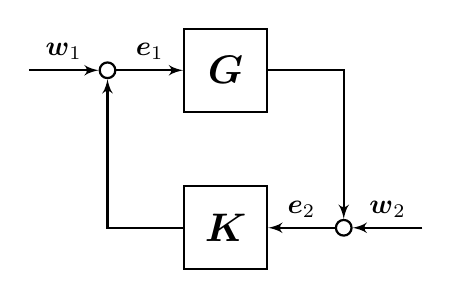
\begin{tikzpicture}[auto, node distance=2cm, >=latex', thick]

        \tikzstyle{block} = [draw, rectangle, minimum height=3em, minimum width=3em]
        \tikzstyle{sum} = [draw, circle, inner sep=2pt, node distance=2cm]
        \tikzstyle{input} = [coordinate]
        \tikzstyle{output} = [coordinate]

        \node [block] (G) {\Large $\boldsymbol{G}$};
        
        \node [block, below of=G, node distance=2cm] (K) {\Large $\boldsymbol{K}$};
        
        \node [sum, left of=G, node distance=1.5cm] (sum1) {};
        
        \node [sum, right of=K, node distance=1.5cm] (sum2) {};

        \node [input, left of=sum1, node distance=1cm] (w1) {};
        \node [input, right of=sum2, node distance=1cm] (w2) {};
    

        \draw [->] (w1) -- node {$\boldsymbol{w}_1$} (sum1);
        \draw [->] (sum1) -- node {$\boldsymbol{e}_1$} (G);

        \draw [->] (G) -| (sum2);
        \draw [->] (w2) -- node [above] {$\boldsymbol{w}_2$} (sum2);
        \draw [->] (sum2) -- node [above] {$\boldsymbol{e}_2$} (K);
        
        \draw [->] (K) -| (sum1);
    
    \end{tikzpicture}
    \caption{Feedback control loop.}
    \label{fig:control_loop}
\end{figure}

Consider now the plant perturbed by additive uncertainty. The perturbed plant equation is:
\begin{equation}
    \boldsymbol{G}_{p} = \boldsymbol{G} + \boldsymbol{W}_{1}\boldsymbol{\Delta}\boldsymbol{W}_2
\end{equation}
To ensure robust stability of this system, it's necessary to compute $\gamma$ such that:
\begin{equation}
    \| \boldsymbol{W}_2 \boldsymbol{K} \boldsymbol{S}_0 \boldsymbol{W}_1 \|_\infty = \| \boldsymbol{W}_2 \boldsymbol{K}(\boldsymbol{I} + \boldsymbol{G}\boldsymbol{K}(s))^{-1}  \boldsymbol{W}_1 \|_\infty \leq \gamma
\end{equation}
The perturbation $\boldsymbol{\Delta}$ has to satisfy $\|\boldsymbol{\Delta}\|<\frac{1}{\gamma}$, which therefore represents a stability margin for the system.
In order to find this margin and the frequency in which the worst-case perturbation occurs, we can use the MATLAB function \texttt{hinfnorm}. Using this procedure, the margin found was $\frac{1}{\gamma} = 0.0611$ at frequency $\omega=$ \SI[per-mode=fraction]{2.8327}{\radian\per\second}.

Then, we can use the function \texttt{sigma} to plot the Singular Values as function of frequency and overlay the worst-case found. The resulting plot is shown in Figure \ref{fig:SV_add}.

\begin{figure}[htb]
  \centering
  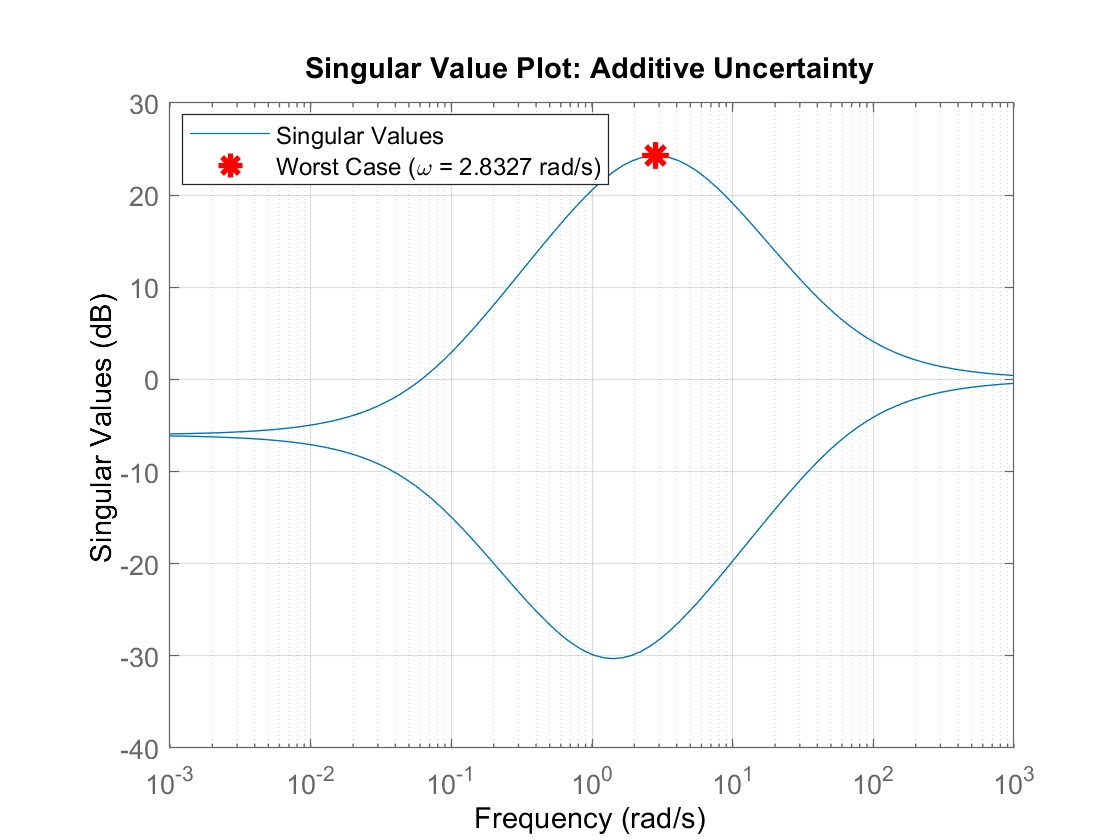
\includegraphics[scale=0.3]{images/Singular_Value_plot_Additive_uncertainty.jpg}
  \caption{Singular Value plot for the system with additive uncertainty.}
  \label{fig:SV_add}
\end{figure}

Instead, if we have multiplicative output uncertainty the process is quite similar. The perturbed plant equation is:

\begin{equation}
    \boldsymbol{G}_{p} = (\boldsymbol{I}+\boldsymbol{W}_{1}\boldsymbol{\Delta}\boldsymbol{W}_2)\boldsymbol{G}
\end{equation}

In this case, for robust stability we have to compute $\gamma$:
\begin{equation}
    \| \boldsymbol{W}_2 \boldsymbol{T}_0 \boldsymbol{W}_1 \|_\infty = \| \boldsymbol{W}_2 \boldsymbol{G} \boldsymbol{K}(\boldsymbol{I} + \boldsymbol{G}\boldsymbol{K}(s))^{-1}  \boldsymbol{W}_1 \|_\infty \leq \gamma
\end{equation}

And again, the perturbation $\boldsymbol{\Delta}$ has to satisfy $\|\boldsymbol{\Delta}\|<\frac{1}{\gamma}$. In this case, the margin found was $\frac{1}{\gamma} = 0.0612$ at frequency $\omega=$ \SI[per-mode=fraction]{2.8270}{\radian\per\second}, which are very close to the previous case. The resulting Singular Value plot is shown in Figure \ref{fig:SV_mult}.

\begin{figure}[htb]
  \centering
  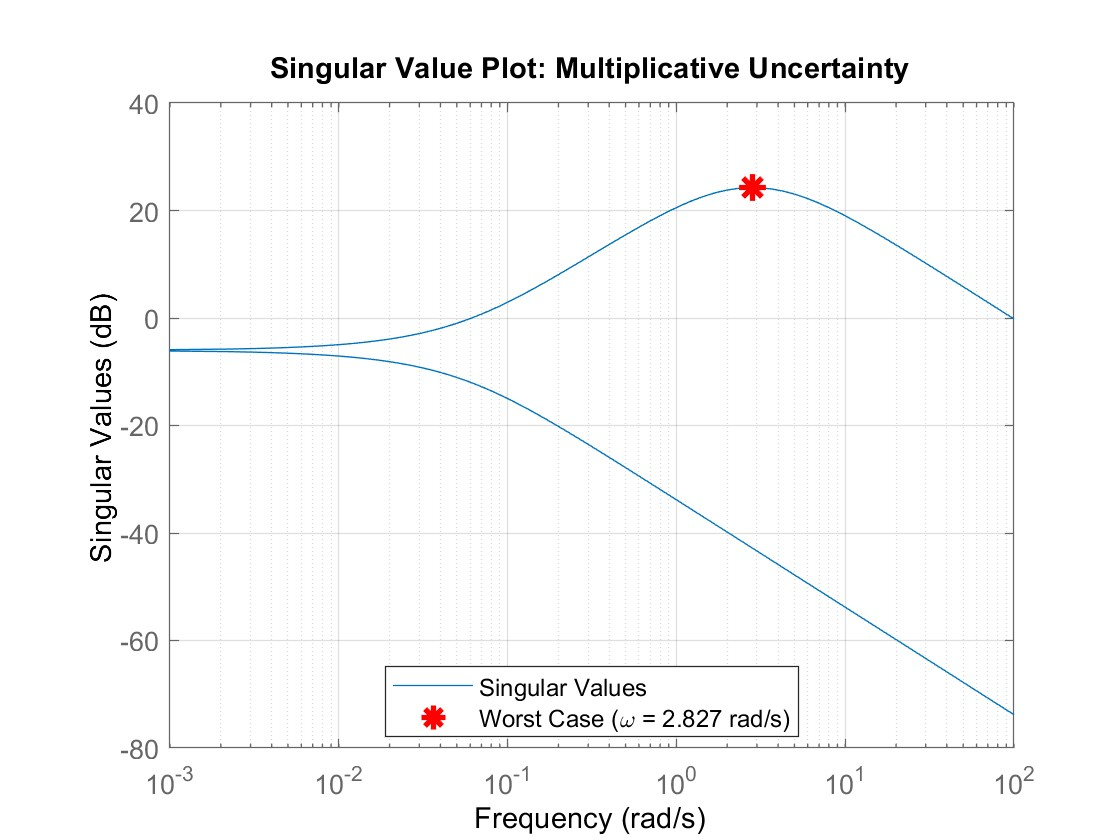
\includegraphics[scale=0.3]{images/Singular_Value_plot_Multiplicative_uncertainty.jpg}
  \caption{Singular Value plot for the system with multiplicative uncertainty.}
  \label{fig:SV_mult}
\end{figure}

The procedure explained in chapter 8.6.1 of \cite{Sko05} shows how to find the smallest destabilizing perturbation of a system, which satisfies $\|\boldsymbol{\Delta}'\|_{\infty}=1/\gamma$. The formula is:

\begin{equation}
    \boldsymbol{\Delta'} = - \frac{1}{\gamma}\boldsymbol{V}\boldsymbol{U}^H
    \label{eq:smallest_dest_pert}
\end{equation}

This returns a matrix such that  $\bar{\sigma}(\Delta'(j\omega^*)) = 1/\gamma$. Since it was required that the greatest singular value was equal to gamma, the term $1/\gamma$ in Eq. \ref{eq:smallest_dest_pert} was substituted with $\gamma$. This was done for both the additive and multiplicative uncertainty, yielding a system which is not stable, and therefore not in $\mathcal{RH}_{\infty}$. This was proved by confirming that the matrices of \ref{eq:int_stab_check} had poles in the open right-half plane by using the two perturbed plants in the place of $\boldsymbol{G}(s)$. The procedure and results discussed in this section can be found in code \texttt{Ex\_2\_1\_3.m}.



\chapter{MIMO-Systems}

\section{Proof of equivalence}
Given a system in general control configuration with generalized plant $\boldsymbol{P}$ and controller $\boldsymbol{K}$, suppose the exogenous input $\boldsymbol{w}$ is white noise with unit intensity. That is:
\begin{equation}
    E \left \{\boldsymbol{w}(t)\boldsymbol{w}(\tau)^T \right\} =\boldsymbol{I}\delta (t-\tau)
    \label{eq:exp_w}
\end{equation}

The error signal is given by:

\begin{equation}
    \boldsymbol{z} = \mathcal{F}_l(\boldsymbol{P},\boldsymbol{K})\boldsymbol{w}=\boldsymbol{F}\boldsymbol{w}
\end{equation}

The expected power in the error signal $\boldsymbol{z}$ is then given by:

\begin{equation}
    E\left\{ \lim_{T\rightarrow \infty} \frac{1}{2T} \int_{-T}^{T} \boldsymbol{z}(t)^T\boldsymbol{z}(t) \, dt \right\} = E\left\{ \lim_{T\rightarrow \infty} \frac{1}{2T} \int_{-T}^{T} \text{trace}\left [\boldsymbol{z}(t)^T\boldsymbol{z}(t)\right] dt \right\}
\end{equation}

Which are equivalent because $\boldsymbol{z}(t)^T\boldsymbol{z}(t)$ is a scalar. The following step was not proved but it's assumed that, under certain conditions, it's possible to move the expected value inside both the limit and the integral, revealing the autocorrelation function $R_{zz}$:

\begin{equation}
    \lim_{T\rightarrow \infty} \frac{1}{2T} \int_{-T}^{T} \text{trace} \left\{ E \left[ \boldsymbol{z}(t)^T\boldsymbol{z}(t) \right] \right\} dt =\lim_{T\rightarrow \infty} \frac{1}{2T} \int_{-T}^{T} \text{trace} \left[ R_{zz}(t,t) \right] dt
\end{equation}

The auto-correlation at time instant $t$ can be written by using the convolutional integral:

\begin{equation}
    \begin{aligned}
        R_{zz}(t,t) &= E\left\{ \left( \int_{-\infty}^{\infty} \mathbf{H}(\tau_1) \boldsymbol{\omega}(t-\tau_1) \, d\tau_1 \right) \cdot \left( \int_{-\infty}^{\infty} \mathbf{H}(\tau_2) \boldsymbol{\omega}(t-\tau_2) \, d\tau_2 \right)^T \right\} \\
        &= \int_{-\infty}^{\infty} \int_{-\infty}^{\infty} \mathbf{H}(\tau_1) E \left[ \boldsymbol{\omega}(t-\tau_1) \boldsymbol{\omega}^T(t-\tau_2) \right] \mathbf{H}^T(\tau_2) \, d\tau_1 \, d\tau_2
    \end{aligned}
\end{equation}

Where the last step is possible because the impulse response matrix is deterministic. By using the hypothesis in Eq. \ref{eq:exp_w},

\begin{equation}
    \int_{-\infty}^{\infty} \int_{-\infty}^{\infty} \mathbf{H}(\tau_1) \mathbf{I} \delta(\tau_2 - \tau_1) \mathbf{H}^T(\tau_2) \, d\tau_1 \, d\tau_2
\end{equation}

Which proves how the autocorrelation of $\boldsymbol{z}$ is not time-dependent and therefore can be brought out of the integral and limit.

By substituting this into the previous equation:

\begin{align}
&\lim_{T\rightarrow \infty} \frac{1}{2T}  \int_{-T}^{T} \underbrace{ \operatorname{trace} \left\{ E \left[ (\mathbf{z}(t) \mathbf{z}(t))^T \right] \right\} }_{\text{NOT TIME DEP.}} dt = \\
&= \lim_{T\rightarrow \infty} \frac{1}{2T} \cdot 2T \cdot \operatorname{trace} (R_{zz}(t,t)) = \\[10pt]
&= \operatorname{trace} E \left[ (\mathbf{z}(t) \mathbf{z}(t))^T \right]
\end{align}

By using the equation of $R_{zz}$, this is equivalent to:

\begin{align}
&= \operatorname{trace} \left\{ \int_{-\infty}^{\infty} \int_{-\infty}^{\infty} \mathbf{H}(\tau_1) \mathbf{I} \delta(\tau_2 - \tau_1) \mathbf{H}^T(\tau_2) \, d\tau_1 \, d\tau_2 \right\} = \\
&= \operatorname{trace} \left\{ \int_{-\infty}^{\infty} \mathbf{H}(\tau_1) \mathbf{I} \left( \int_{-\infty}^{\infty} \delta(\tau_2 - \tau_1) \mathbf{H}^T(\tau_2) \, d\tau_2 \right) d\tau_1 \right\} = \\
&= \operatorname{trace} \left\{ \int_{-\infty}^{\infty} \mathbf{H}(\tau_1) \mathbf{H}^T(\tau_1) \, d\tau_1 \right\} \\
\end{align}

By Parseval's theorem, it's possible to move to the frequency domain equivalent:

\begin{align}
&= \operatorname{trace} \left\{ \frac{1}{2\pi} \int_{-\infty}^{\infty} \mathbf{F}(j\omega) \mathbf{F}^H(j\omega) \, d\omega \right\} = \\
&= \frac{1}{2\pi} \int_{-\infty}^{\infty} \operatorname{trace} \left[ \mathbf{F}(j\omega) \mathbf{F}^H(j\omega) \right] d\omega = \|\mathbf{F}\|_2^2 = \|\mathbf{F}_l(\mathbf{P}, \mathbf{K})\|_2^2
\end{align}

Where the definition of $\mathcal{H}_2$ norm of a system and the definition of $\boldsymbol{F}$ have been used.
This proves that by minimizing the $\mathcal{H}_2$ norm of $\boldsymbol{F}$, we are minimizing the root mean square value of $\boldsymbol{z}$ under unit intensity white noise input, as discussed in \cite{Sko05}.


\section{System zero and down squaring}
Given the following state-space system:

\begin{align*}
\dot{\boldsymbol{x}} &= \begin{bmatrix} 2 & 0 \\ 0 & -2 \end{bmatrix} \boldsymbol{x} + \begin{bmatrix} 1 & 0 \\ 0 & 1 \end{bmatrix} \boldsymbol{u} \\
y &= \begin{bmatrix} 1 & -1 \end{bmatrix} \boldsymbol{x} + \begin{bmatrix} 1 & 1 \end{bmatrix} \boldsymbol{u}
\end{align*}

Whose transfer function matrix is:

\begin{equation}
    \boldsymbol{G}(s)=\frac{1}{(s-2)(s+2)} \begin{bmatrix}
        (s-1)(s+2) & (s+1)(s-2)
    \end{bmatrix}
\end{equation}

From this formulation, it's easy to see that the zero polynomial (as defined previously) is $z(s)=1$, meaning we don't have any transmission zeros. If we add a pre-compensator of the type $\boldsymbol{k}=\begin{bmatrix}
    k_1 \\ k_2
\end{bmatrix}$, the state-space system becomes:

\begin{align}
\dot{\boldsymbol{x}} &= \begin{bmatrix} 2 & 0 \\ 0 & -2 \end{bmatrix} \boldsymbol{x} + \begin{bmatrix} 1 & 0 \\ 0 & 1 \end{bmatrix} \boldsymbol{k}v \\
y &= \begin{bmatrix} 1 & -1 \end{bmatrix} \boldsymbol{x} + \begin{bmatrix} 1 & 1 \end{bmatrix} \boldsymbol{k}v
\end{align}

where $\boldsymbol{u}=\boldsymbol{k}v$. The transfer function becomes one-dimensional:

\begin{equation}
    G(s)=\frac{(k_1+k_2)s^2+(k_1-k_2)s-2(k_1+k_2)}{(s-2)(s+2)}
\end{equation}

The zeros of the system are the roots of Eq. \ref{eq:zeros_pol}:
\begin{equation}
    (k_1+k_2)s^2+(k_1-k_2)s-2(k_1+k_2)=as^2+bs+c=0
    \label{eq:zeros_pol}
\end{equation}

It's simple to prove that the two roots $s_1$ and $s_2$ of the second degree polynomial satisfy the equation:

\begin{equation}
    s_1\cdot s_2 = \frac{c}{a}= \frac{-2(k_1+k_2)}{(k_1+k_2)}=-2
\end{equation}

This means that the product of the two zeros is negative, and therefore it is impossible to place both the zeros of the system in the same open half of the complex plane. The transmission zeros computed for this system with the procedure explained in section 1.1 for non-square system can be seen in the code \texttt{Ex\_2\_2\_2.m}.

\section{Stabilization via Youla-controller}
Following the procedure from ACS, Exercise 07, a stabilizing Youla controller was designed by finding a coprime factorization using:

\begin{equation}
    \begin{bmatrix}
        \mathbf{M} & \mathbf{U} \\
        \mathbf{N} & \mathbf{V}
    \end{bmatrix}
    \stackrel{s}{=}
    \left[
    \begin{array}{c|c}
        \mathbf{A} + \mathbf{B}\mathbf{F} & \begin{bmatrix} \mathbf{B} & -\mathbf{H} \end{bmatrix} \\
        \hline
        \begin{bmatrix} \mathbf{F} \\ \mathbf{C} + \mathbf{D}\mathbf{F} \end{bmatrix} & \begin{bmatrix} \mathbf{I} & \mathbf{0} \\ \mathbf{D} & \mathbf{I} \end{bmatrix}
    \end{array}
    \right],
\end{equation}

Where $\boldsymbol{F}$ and $\boldsymbol{H}$ were found by using the MATLAB \texttt{place} function. The poles were placed in $\begin{bmatrix}-2,-5,-8\end{bmatrix}$. If needed, they can be moved further to the left of the complex plane to make the response of the system faster:

\begin{center}
    \centering
    \begin{verbatim}
            F = -place(A, B, [-2 -5 -8]);
            H = -transpose(place(A' , C' , [ -2 -5 -8]));
    \end{verbatim}
\end{center}

The obtained coprime factors are:
\begin{align}
    M(s) &= \frac{(s-2)(s+2)(s+1)}{(s+8)(s+5)(s+2)} \\[1ex]
    N(s) &= \frac{s-1}{(s+8)(s+5)(s+2)} \\[1ex]
    U(s) &= \frac{-6664(s+2)(s+0.9412)}{(s+8)(s+5)(s+2)} \\[1ex]
    V(s) &= \frac{(s-7.704)(s^2 + 36.7s + 614.8)}{(s+8)(s+5)(s+2)}
\end{align}

The stabilizing controllers are parametrized through the transfer function $\boldsymbol{Q}\in\mathcal{RH}_\infty$:

\begin{equation}
    \boldsymbol{K} = -(\boldsymbol{V} + \boldsymbol{Q}\boldsymbol{N})^{-1}(\boldsymbol{U} + \boldsymbol{Q}\boldsymbol{M})
\end{equation}

By setting $\boldsymbol{Q}=\boldsymbol{0}$, the resulting controller has the following transfer function:
\begin{equation}
    K(s) = \frac{6664 (s+2) (s+0.9412)}{(s-7.704) (s^2 + 36.7s + 614.8)}
\end{equation}

Since the system is SISO, to check stability it is only necessary to check one transfer function. In particular, we have to check that the poles of $(1+GK)^{-1}$ lie in the closed-LHP. The poles have been computed as the roots of the pole polynomial, and only stable poles were found. The step response of the system is shown in Figure \ref{fig:Youla_par_resp}. The procedure and results described in this section can be found in the code \texttt{Ex\_2\_2\_3.m}.

\begin{figure}[htb]
  \centering
  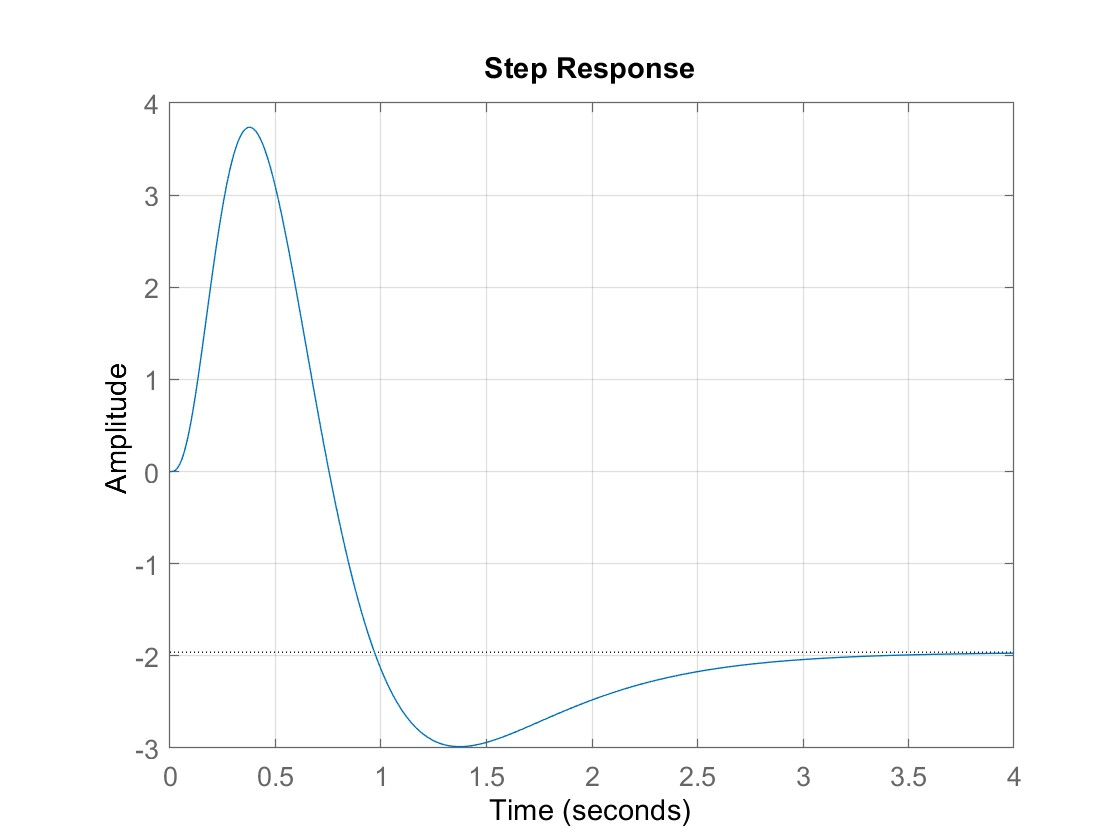
\includegraphics[scale=0.25]{images/Youla_par_sys_res.jpg}
  \caption{System response with Youla-controller.}
  \label{fig:Youla_par_resp}
\end{figure}


\chapter{Stability and LFT}
\section{Stability and LFT}
Given the following dynamical system:

\begin{equation}
    \begin{aligned}
    % State Equation
        \begin{bmatrix}
        \dot{x}_1 \\
        \dot{x}_2
        \end{bmatrix}
        &=
        \begin{bmatrix}
        0 & 1 \\
        -\frac{k_p}{m_p} & -\frac{c_p}{m_p}
        \end{bmatrix}
        \begin{bmatrix}
        x_1 \\
        x_2
        \end{bmatrix}
        +
        \begin{bmatrix}
        0 \\
        \frac{1}{m_p}
        \end{bmatrix}
        u \\
        \\
        % Output Equation
        y &=
        \begin{bmatrix}
        h_p & 0
        \end{bmatrix}
        \begin{bmatrix}
        x_1 \\
        x_2
        \end{bmatrix}
    \end{aligned}
\end{equation}

Where $m_p, c_p, ,k_p$ and $h_p$ are uncertain parameters described in Table \ref{tab:parameters}.

\begin{table}[h]
\centering
\begin{tabular}{|c|c|c|c|}
\hline
\textbf{Parameter} & \textbf{Minimum Value} & \textbf{Nominal Value} & \textbf{Maximum Value} \\ \hline
$m$ & 5   & 10  & 18  \\ \hline
$c$ & 6   & 10  & 14  \\ \hline
$k$ & 0.8 & 1   & 1.8 \\ \hline
$h$ & 2.0 & 2.5 & 4.5 \\ \hline
\end{tabular}
\caption{Parameter Uncertainty Ranges}
\label{tab:parameters}
\end{table}

It's possible to parametrize this uncertainty as a function of four uncertainty channels $\Delta_m, \Delta_c, \Delta_k$ and $\Delta_h$ for asymmetric ranges. For example, we can write $k_p$ as:

\begin{equation}
    k_p = \frac{a+b\Delta_k}{c+d\Delta_k}
\end{equation}

where $a, b, c$ and $d$ are determined by imposing:

\begin{equation}
    \left\{
    \begin{aligned}
    \Delta_k &= -1 & \quad k_p &= k_{\text{min}} \\
    \Delta_k &= 0  & \quad k_p &= k_{\text{nom}} \\
    \Delta_k &= 1  & \quad k_p &= k_{\text{max}}
    \end{aligned}
    \right.
\end{equation}

This is not enough equations to determine all four variables, so $c$ is arbitrarily fixed to $1$. The same can be done for all other parameters, including $c_p$ which has a symmetric range. The results are the following:

\begin{equation}
    \begin{aligned}
        m_p = \frac{10+3.846\Delta_m}{1-0.231\Delta_m}\\
        c_p = c_{\text{nom}}(1+0.4\Delta_c)\\
        k_p=\frac{1-0.28\Delta_k}{1-0.6\Delta_k}\\
        h_p=\frac{2.5-0.7\Delta_h}{1-0.6\Delta_h}
    \end{aligned}
\end{equation}

Having obtained the parametrization of the uncertainties, it's possible to re-write them as the LFT between a matrix $\boldsymbol{M}_i$ and the uncertainty $\Delta_i$ (except for $c_p$). For the general case:

\begin{equation}
\begin{aligned}
\frac{a}{c + d\Delta_i} + \frac{b\Delta_i}{c + d\Delta_i} 
&= \frac{a}{c} \frac{1 + d\Delta_i/c - d\Delta_i/c}{1 + d\Delta/c} + \frac{b\Delta_i/c}{1 + d\Delta_i/c} \\
&= \frac{a}{c} - \frac{a}{c} \frac{d\Delta_i/c}{1 + d\Delta_i/c} + \frac{b\Delta_i/c}{1 + d\Delta_i/c} \\
&= \frac{a}{c} + \left( b - \frac{ad}{c} \right) \Delta_i \left( 1 + \frac{d\Delta_i}{c} \right)^{-1} \cdot \frac{1}{c}
\end{aligned}
\end{equation}

The upper LFT is defined as:
\begin{equation}
    \mathcal{F}_u(\boldsymbol{M}_i, \boldsymbol{\Delta}_i) := \boldsymbol{M}_{i,22} + \boldsymbol{M}_{i,21}\boldsymbol{\Delta}_i(\boldsymbol{I} - \boldsymbol{M}_{i,11}\boldsymbol{\Delta}_i)^{-1}\boldsymbol{M}_{i,12}
\end{equation}

Therefore, in this case, matrix $\boldsymbol{M}_i$ is defined as:

\begin{equation}
    \boldsymbol{M}_i = \begin{bmatrix}
        -\frac{d}{c} & \frac{1}{c} \\
        b-\frac{ad}{c} & \frac{a}{c}
    \end{bmatrix}
\end{equation}

This was performed for the uncertainties $m_p, k_p$ and $h_p$. In particular, since $m_p$ always appears at the denominator, the parametrization was performed on $1/m_p$. The results are the following:

\begin{equation}
    \begin{aligned}
        \boldsymbol{M}_m &= \begin{bmatrix} -0.3846 & 0.1 \\ -0.6156 & 0.1 \end{bmatrix} \\
        \\
        \boldsymbol{M}_k &= \begin{bmatrix} 0.6 & 1 \\ 0.32 & 1 \end{bmatrix} \\
        \\
        \boldsymbol{M}_h &= \begin{bmatrix} 0.6 & 1 \\ 0.8 & 2.5 \end{bmatrix}
    \end{aligned}
\end{equation}

The new block diagram of this system can be now drawn and is shown in Figure \ref{fig:uncertainty_block_diag}.


\begin{figure}
    \centering
    \resizebox{\textwidth}{!}{
    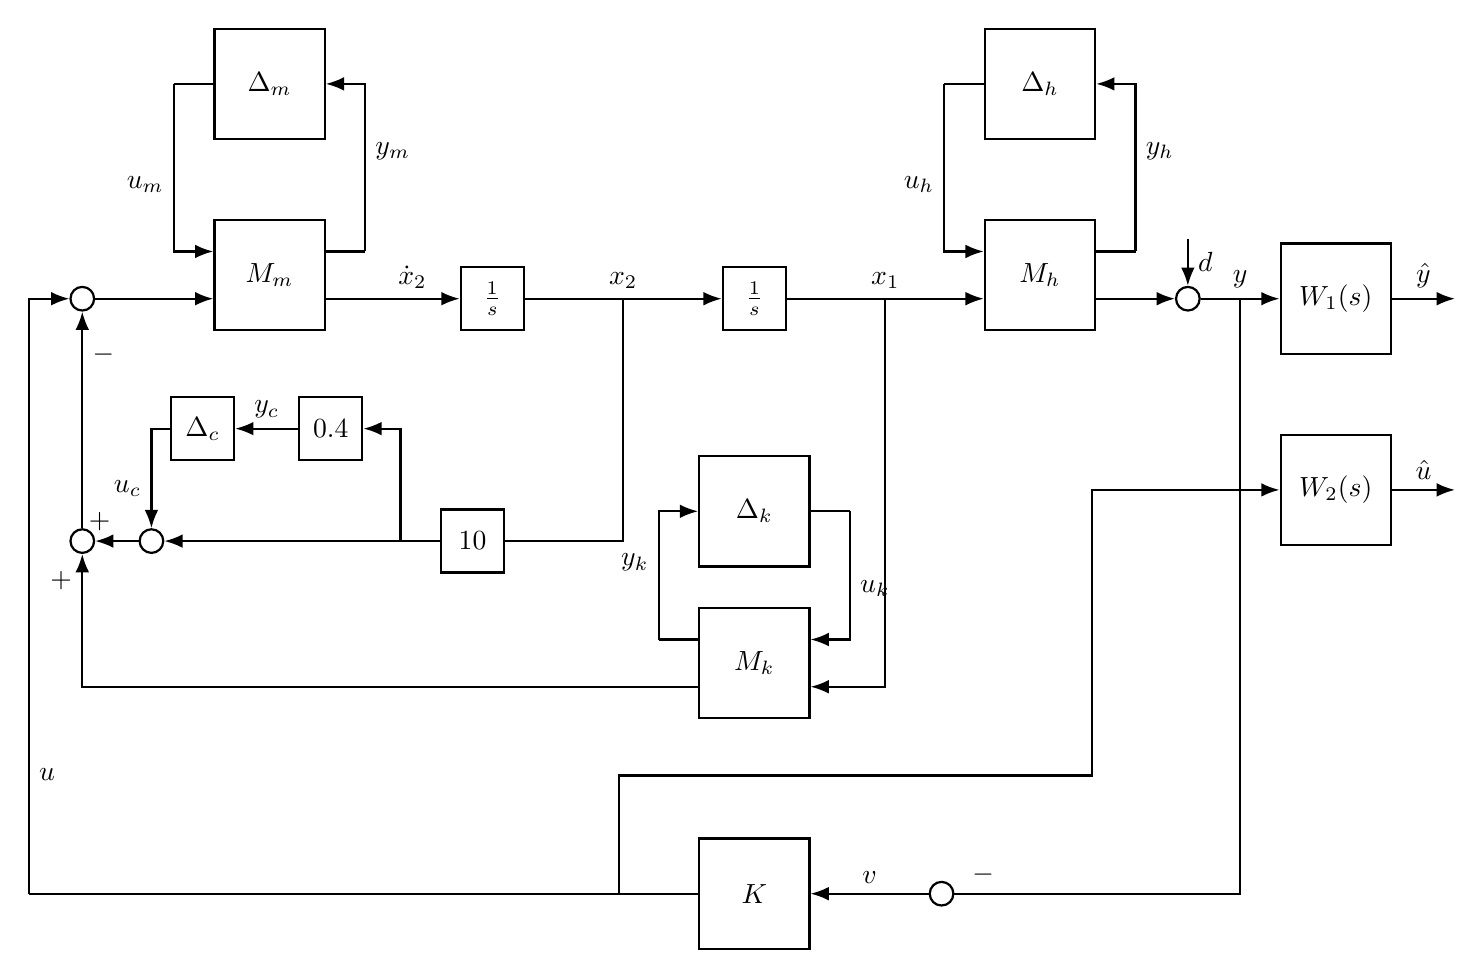
\begin{tikzpicture}[
    auto,
    node distance=1.2cm,
    >=Latex,
    block/.style={draw, rectangle, minimum height=1.4cm, minimum width=1.4cm, align=center, thick},
    smallblock/.style={draw, rectangle, minimum height=0.8cm, minimum width=0.8cm, align=center, thick},
    sum/.style={draw, circle, inner sep=1pt, minimum size=3mm, thick},
    connector/.style={->, thick},
    line/.style={thick},
    point/.style={fill, circle, minimum size=3pt, inner sep=0pt}
]

    \node [smallblock] (int1) at (3,0) {$\frac{1}{s}$};
    \node [smallblock, right=2.5cm of int1] (int2) {$\frac{1}{s}$};


    \node [block, left=1.7cm of int1, yshift=0.3cm] (Mm) {$M_m$};


    \coordinate (mm_in_main) at ($(Mm.west)-(0,0.3)$);
    \node [sum, left=1.5cm of mm_in_main] (sum1) {}; 


    \node [block, above=1.0cm of Mm] (Dm) {$\Delta_m$};


    \node [block, right=2.5cm of int2, yshift=0.3cm] (Mh) {$M_h$};
    \node [sum, right=1.0cm of Mh, yshift=-0.3cm] (sum_d) {};
    \node [block, right=1.0cm of sum_d] (W1) {$W_1(s)$};
    \node [coordinate, right=0.8cm of W1] (y_hat) {};
    \node [block, above=1.0cm of Mh] (Dh) {$\Delta_h$};


    \coordinate (u_m_in) at ($(Mm.west)+(0,0.3)$);
    \coordinate (m_in) at ($(Mm.west)-(0,0.3)$);
    

    \coordinate (y_m_out) at ($(Mm.east)+(0,0.3)$);
    \coordinate (m_out) at ($(Mm.east)-(0,0.3)$);


    \coordinate (u_h_in) at ($(Mh.west)+(0,0.3)$);
    \coordinate (h_in) at ($(Mh.west)-(0,0.3)$);
    

    \coordinate (y_h_out) at ($(Mh.east)+(0,0.3)$);
    \coordinate (h_out) at ($(Mh.east)-(0,0.3)$);


    \draw [connector] (sum1) -- (m_in);
    
    \draw [connector] (m_out) -- ++(0.5,0) |- node [near end, above] {$\dot{x}_2$} (int1);


    \draw [connector] (int1) -- node [above] (x2) {$x_2$} (int2);
    \draw [connector] (int2) -- node [above] (x1) {$x_1$} (h_in);
    \draw [connector] (h_out) -- (sum_d);
    \draw [connector] (sum_d) -- node [above] (y) {$y$} (W1);
    \draw [connector] (W1) -- node [above] {$\hat{y}$} (y_hat);
    

    \draw [connector] ($(sum_d.north)+(0,0.6)$) -- node [right] {$d$} (sum_d.north);


    \draw [line] (y_m_out) -- ++(0.5,0) coordinate (ym_turn);
    \draw [connector] (ym_turn) |- node[right, pos=0.3] {$y_m$} (Dm.east);

    \draw [line] (Dm.west) -- ++(-0.5,0) coordinate (um_turn);
    \draw [connector] (um_turn) |- node[left, pos=0.3] {$u_m$} (u_m_in);

   
    \draw [line] (y_h_out) -- ++(0.5,0) coordinate (yh_turn);
    \draw [connector] (yh_turn) |- node[right, pos=0.3] {$y_h$} (Dh.east);

    \draw [line] (Dh.west) -- ++(-0.5,0) coordinate (uh_turn);
    \draw [connector] (uh_turn) |- node[left, pos=0.3] {$u_h$} (u_h_in);


    \node [sum, below=2.5cm of Mm, xshift=-1.5cm] (sum_c) {};
    \node [smallblock, right=3.5cm of sum_c] (gain10) {10};
    \node [smallblock, above=0.6cm of gain10, xshift=-1.8cm] (gain04) {0.4};
    \node [smallblock, left=0.8cm of gain04] (Dc) {$\Delta_c$};


    \coordinate (drop_c) at ($(gain10.west)-(0.5,0)$);
    \draw [line] (x2) |- (gain10.east);
    \draw [connector] (gain10.west) -- (sum_c.east);
    \draw [connector] (drop_c) |- (gain04.east);
    \draw [connector] (gain04.west) -- node[above] {$y_c$} (Dc.east);
    \draw [connector] (Dc.west) -| node[left, pos=0.8] {$u_c$} (sum_c.north);



    \node [block, below=3.5cm of int2] (Mk) {$M_k$};
    \node [block, above=0.5cm of Mk] (Dk) {$\Delta_k$};


    \coordinate (u_k_in) at ($(Mk.east)+(0,0.3)$);
    \coordinate (k_in) at ($(Mk.east)-(0,0.3)$);
    

    \coordinate (y_k_out) at ($(Mk.west)+(0,0.3)$);
    \coordinate (k_out) at ($(Mk.west)-(0,0.3)$);

    \draw [line] (x1) |- ($(k_in)+(0.5,0)$) coordinate (drop_k) {};
    \draw [connector] (drop_k) -- (k_in);


    \node [sum] (sum_out) at (sum1 |- sum_c) {};

    \draw [connector] (k_out) -| node[pos=0.9,left] {$+$} (sum_out.south);
    \draw [connector] (sum_c.west) -- node[pos=0.9, above] {$+$} (sum_out.east);
    \draw [connector] (sum_out.north) -| node[pos=0.9, right] {$-$} (sum1.south);
    

    \draw [line] (y_k_out) -- ++(-0.5,0) coordinate (yk_turn);
    \draw [connector] (yk_turn) |- node[left, pos=0.3] {$y_k$} (Dk.west);


    \draw [line] (Dk.east) -- ++(0.5,0) coordinate (uk_turn);
    \draw [connector] (uk_turn) |- node[right, pos=0.3] {$u_k$} (u_k_in);


    \node [block, below=1.5cm of Mk] (K) {$K$};
    \node [block, below=1cm of W1] (W2) {$W_2(s)$};
    \node [coordinate, right=0.8cm of W2] (u_hat) {};

    \node [sum, right=1.5cm of K] (y_v) {};

    \draw [line] (y) |- node[above, pos=0.95] {$-$} (y_v.east);
    \draw [connector] (y_v.west) -- node[above, pos=0.5] {$v$} (K.east);
    \draw [line] (K.west) -- ++(-8.5,0) coordinate (u_path);
    \draw [connector] (u_path) |- node[right, pos=0.1] {$u$} (sum1.west);
    \draw [connector] (K.west) -- ++(-1,0) -- ++(0,1.5) -- ++(6,0) |- (W2.west);
    \draw [connector] (W2.east) -- node[above] {$\hat{u}$} (u_hat);

\end{tikzpicture}
}
    \caption{Block diagram after uncertainty extraction.}
    \label{fig:uncertainty_block_diag}
\end{figure}

From here it's possible to re-arrange the system to an $\Delta$-$P$-$K$ structure shown in Figure \ref{fig:Delta-P-K}. $\boldsymbol{P}$ has to be a system such that:
\begin{equation}
    \begin{bmatrix}
        y_m\\y_c\\y_k\\y_h\\
        \hat{y}\\\hat{u}\\v
    \end{bmatrix}=\boldsymbol{P} \begin{bmatrix}
        u_m\\u_c\\u_k\\u_h\\d\\u
    \end{bmatrix}
\end{equation}


Where $\hat{y}$ and $\hat{u}$ are the output $y$ and input $u$ scaled by the weighting functions $W_1(s)$ and $W_2(s)$, respectively.
By looking at the block diagram, such system can be derived. Here it's the state-space representation:

\begin{align*}
\begin{bmatrix}
\dot{x}_1 \\
\dot{x}_2 \\
\dot{z}_y \\
\dot{z}_u
\end{bmatrix} &= \boldsymbol{A} \begin{bmatrix}
x_1 \\
x_2 \\
z_y \\
z_u
\end{bmatrix} + \boldsymbol{B} \begin{bmatrix}
        u_m\\u_c\\u_k\\u_h\\d\\u
    \end{bmatrix} \\
\begin{bmatrix}
        y_m\\y_c\\y_k\\y_h\\
        \hat{y}\\\hat{u}\\v
    \end{bmatrix} &= \boldsymbol{C} \begin{bmatrix}
x_1 \\
x_2 \\
z_y \\
z_u
\end{bmatrix} + \boldsymbol{D} \begin{bmatrix}
        u_m\\u_c\\u_k\\u_h\\d\\u
    \end{bmatrix}
\end{align*}

\noindent where:

\[
\boldsymbol{A} =
\begin{bmatrix}
0 & 1 & 0 & 0 \\
-M_{m,22}M_{k,22} & -M_{m,22}\bar{c} & 0 & 0 \\
B_{w1}M_{h,22} & 0 & A_{w1} & 0 \\
0 & 0 & 0 & A_{w2}
\end{bmatrix}
\]

\[
\boldsymbol{B} =
\begin{bmatrix}
0 & 0 & 0 & 0 & 0 & 0 \\
M_{m,21} & -M_{m,22} & -M_{k,21}M_{m,22} & 0 & 0 & M_{m,22} \\
0 & 0 & 0 & B_{w1}M_{h,21} & B_{w1} & 0 \\
0 & 0 & 0 & 0 & 0 & B_{w2}
\end{bmatrix}
\]

\[
\boldsymbol{C} =
\begin{bmatrix}
-M_{m,12}M_{k,22} & -M_{m,12}\bar{c} & 0 & 0 \\
0 & 0.4\bar{c} & 0 & 0 \\
M_{k,12} & 0 & 0 & 0 \\
M_{h,12} & 0 & 0 & 0 \\
D_{w1}M_{h,22} & 0 & C_{w1} & 0 \\
0 & 0 & 0 & C_{w2} \\
-M_{h,22} & 0 & 0 & 0
\end{bmatrix}
\]

\[
\boldsymbol{D} =
\begin{bmatrix}
M_{m,11} & -M_{m,12} & -M_{m,12}M_{k,21} & 0 & 0 & M_{m,12} \\
0 & 0 & 0 & 0 & 0 & 0 \\
0 & 0 & M_{k,11} & 0 & 0 & 0 \\
0 & 0 & 0 & M_{h,11} & 0 & 0 \\
0 & 0 & 0 & D_{w1}M_{h,21} & D_{w1} & 0 \\
0 & 0 & 0 & 0 & 0 & D_{w2} \\
0 & 0 & 0 & -M_{h,21} & -1 & 0
\end{bmatrix}
\]

\begin{figure}
    \centering
    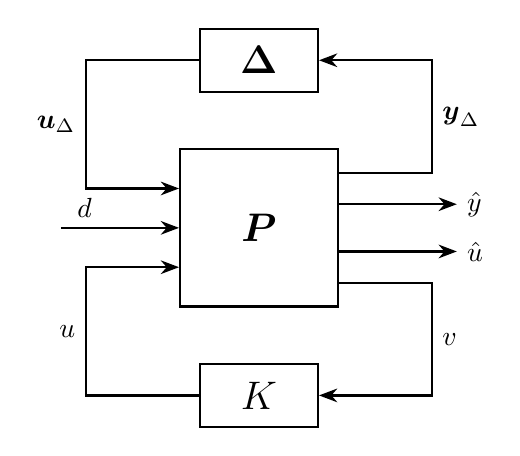
\begin{tikzpicture}[
    >=Stealth,
    thick,
    block/.style={draw, rectangle, minimum height=0.8cm, minimum width=1.5cm, align=center, font=\Large},
    bigblock/.style={draw, rectangle, minimum height=2cm, minimum width=2cm, align=center, font=\Large}
]

    \node[bigblock] (P) {$\boldsymbol{P}$};
    \node[block, above=0.7cm of P] (Delta) {$\boldsymbol{\Delta}$};
    \node[block, below=0.7cm of P] (K) {$K$};


    \coordinate (P_uD)   at ($(P.west) + (0,  0.5)$);
    \coordinate (P_w)    at ($(P.west) + (0,  0)$);
    \coordinate (P_u)    at ($(P.west) + (0, -0.5)$);


    \coordinate (P_yD)   at ($(P.east) + (0,  0.7)$);
    \coordinate (P_y)    at ($(P.east) + (0,  0.3)$);
    \coordinate (P_uhat) at ($(P.east) + (0, -0.3)$);
    \coordinate (P_v)    at ($(P.east) + (0, -0.7)$);


    \coordinate (LeftLine)  at (-2.2, 0);
    \coordinate (RightLine) at ( 2.2, 0);


    \draw[->] ($(P_w) + (-1.5cm, 0)$) -- (P_w) node[pos=0.2, above] {$d$};

    \draw[->] (P_y) -- ($(P_y) + (1.5cm, 0)$) node[right] {$\hat{y}$};
    \draw[->] (P_uhat) -- ($(P_uhat) + (1.5cm, 0)$) node[right] {$\hat{u}$};

    \draw[->] (P_yD) -- (P_yD -| RightLine) coordinate (r_up) |- (Delta.east);
    \path (r_up) -- (r_up |- Delta.east) node[midway, right] {$\boldsymbol{y}_\Delta$};

    \draw[->] (Delta.west) -- (Delta.west -| LeftLine) coordinate (l_up) |- (P_uD);
    \path (l_up) -- (l_up |- P_uD) node[midway, left] {$\boldsymbol{u}_\Delta$};

    \draw[->] (P_v) -- (P_v -| RightLine) coordinate (r_down) |- (K.east);
    \path (r_down) -- (r_down |- K.east) node[midway, right] {$v$};

    \draw[->] (K.west) -- (K.west -| LeftLine) coordinate (l_down) |- (P_u);
    \path (l_down) -- (l_down |- P_u) node[midway, left] {$u$};

\end{tikzpicture}
    \caption{$\Delta$-$P$-$K$ Structure.}
    \label{fig:Delta-P-K}
\end{figure}

The reader may notice how there are two extra states in this system. This is because the two weighting functions are dynamic systems that have as state-space equations:

\begin{equation}
    \begin{aligned}
        \dot{z}_y = A_{w1} z_y + B_{w1} y\\
        \hat{y} = c_{w1} z_y + C_{w1} y
    \end{aligned}
\end{equation}

\begin{equation}
    \begin{aligned}
        \dot{z}_u = A_{w2} z_u + B_{w2} u\\
        \hat{u} = c_{w2} z_u + C_{w2} u
    \end{aligned}
\end{equation}

While the matrix $\boldsymbol{\Delta}$ is defined as:
\begin{equation}
    \boldsymbol{\Delta}=\begin{bmatrix}
        \Delta_m & 0 & 0 & 0\\
        0 & \Delta_c & 0 & 0\\
        0 & 0 & \Delta_c & 0\\
        0 & 0 & 0 & \Delta_h
    \end{bmatrix}
\end{equation}

A similar result could have been obtained through the \textit{Robust Control Toolbox} in MATLAB. Without writing explicitly the uncertainties, the equations of the system are:

\begin{equation}
\begin{aligned}
\begin{bmatrix}
\dot{x}_1 \\
\dot{x}_2 \\
\dot{z}_y \\
\dot{z}_u
\end{bmatrix}
&=
\begin{bmatrix}
0 & 1 & 0 & 0 \\
-\frac{k_p}{m_p} & -\frac{c_p}{m_p} & 0 & 0 \\
B_{w_1}h_p & 0 & A_{w_1} & 0 \\
0 & 0 & 0 & A_{w_2}
\end{bmatrix}
\begin{bmatrix}
x_1 \\
x_2 \\
z_y \\
z_u
\end{bmatrix}
+
\begin{bmatrix}
0 & 0 \\
0 & \frac{1}{m_p} \\
B_{w_1} & 0 \\
0 & B_{w_2}
\end{bmatrix}
\begin{bmatrix}
d \\
u
\end{bmatrix}
\\ \\
\begin{bmatrix}
\hat{y} \\
\hat{u} \\
v
\end{bmatrix}
&=
\begin{bmatrix}
D_{w_1}h_p & 0 & C_{w_1} & 0 \\
0 & 0 & 0 & C_{w_2} \\
-h_p & 0 & 0 & 0
\end{bmatrix}
\begin{bmatrix}
x_1 \\
x_2 \\
z_y \\
z_u
\end{bmatrix}
+
\begin{bmatrix}
D_{w_1} & 0 \\
0 & D_{w_2} \\
-1 & 0
\end{bmatrix}
\begin{bmatrix}
d \\
u
\end{bmatrix}
\end{aligned}
\label{eq:ss_aut}
\end{equation}

Through the function \texttt{ureal}, it's possible to define a uncertain real variable by specifying its range and nominal value.

\begin{center}
    \begin{verbatim}
        m = ureal('m', 10, 'Range', [5, 18]);
        c = ureal('c', 10, 'Range', [6, 14]);
        k = ureal('k', 1, 'Range', [0.8, 1.8]);
        h = ureal('h', 2.5, 'Range', [2, 4.5]);
    \end{verbatim}
\end{center}

Then, Eq.\ref{eq:ss_aut} was written in MATLAB by creating an uncertain state-space system named \texttt{Plant\_aut}. Through the command \texttt{lftdata}, a $P$-$\Delta$ structure was found:

\begin{center}
    \begin{verbatim}
        [P_aut, Delta_aut] = lftdata(Plant_aut);
    \end{verbatim}
\end{center}

Differently from before, where $\boldsymbol{\Delta}$ had four uncertainty channels, with this procedure it has six. This is most likely because MATLAB repeats three times the uncertainty of $m_p$.

A controller was designed to satisfy robust stability and nominal performance. 
The controller designed is the following:
\begin{equation}
    K = \frac{0.3 \left( \frac{s}{0.88729} + 1 \right) \left( \frac{s}{0.1127} + 1 \right) \left( \frac{s}{48} + 1 \right)}{s \left( \frac{s}{2} + 1 \right)^2}
\end{equation}

To check for robust stability, both the plant computed manually and the one computed automatically through the \textit{Robust Control Toolbox}
were rearranged to the $\boldsymbol{M}$-$\boldsymbol{\Delta}$ structure shown in Figure \ref{fig:M-Delta}. This was done in MATLAB by using the \texttt{lft} function by using the following syntax:

\begin{center}
    \begin{verbatim}
        M = lft(P, K);
        M_aut = lft(P_aut, K);
    \end{verbatim}
\end{center}

\begin{figure}
    \centering
    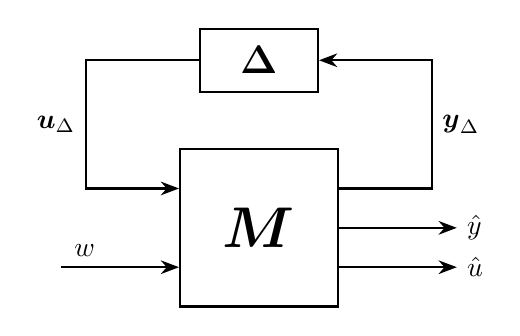
\begin{tikzpicture}[
    >=Stealth,
    thick,
    block/.style={draw, rectangle, minimum height=0.8cm, minimum width=1.5cm, align=center, font=\Large},
    bigblock/.style={draw, rectangle, minimum height=2cm, minimum width=2cm, align=center, font=\huge}
]

    \node[bigblock] (N) {$\boldsymbol{M}$};
    \node[block, above=0.7cm of N] (Delta) {$\boldsymbol{\Delta}$};

    \coordinate (N_uD) at ($(N.west) + (0,  0.5)$);
    \coordinate (N_w)  at ($(N.west) + (0, -0.5)$);

    \coordinate (N_yD)   at ($(N.east) + (0,  0.5)$);
    \coordinate (N_yhat) at ($(N.east) + (0,  0)$);
    \coordinate (N_uhat) at ($(N.east) + (0, -0.5)$);

    \coordinate (LeftLine)  at (-2.2, 0);
    \coordinate (RightLine) at ( 2.2, 0);


    \draw[->] ($(N_w) + (-1.5cm, 0)$) -- (N_w) node[pos=0.2, above] {$w$};

    \draw[->] (N_yhat) -- ($(N_yhat) + (1.5cm, 0)$) node[right] {$\hat{y}$};
    \draw[->] (N_uhat) -- ($(N_uhat) + (1.5cm, 0)$) node[right] {$\hat{u}$};

    \draw[->] (N_yD) -- (N_yD -| RightLine) coordinate (r_up) |- (Delta.east);
    \path (r_up) -- (r_up |- Delta.east) node[midway, right] {$\boldsymbol{y}_\Delta$};

    \draw[->] (Delta.west) -- (Delta.west -| LeftLine) coordinate (l_up) |- (N_uD);
    \path (l_up) -- (l_up |- N_uD) node[midway, left] {$\boldsymbol{u}_\Delta$};

\end{tikzpicture}
    \caption{$M$-$\Delta$ Structure.}
    \label{fig:M-Delta}
\end{figure}

Robust stability is satisfied for the small gain theorem if:

\begin{equation}
    \|\boldsymbol{M}_{11}\|_{\infty}\leq 1
    \label{eq:robust_stability_req}
\end{equation}

Unfortunately, for both types of uncertainty modeling, this requirement is not satisfied. The norm in the two cases is $3.46$ and $11.10$, respectively. Due to the increased number of uncertainty channels, the system obtained using the \textit{Robust Control Toolbox} has more conservatism, as it can be seen by the increased norm.

Another degree of conservatism is introduced by Eq. \ref{eq:robust_stability_req}. This constraint doesn't consider the type of uncertainty the system is subject to. To account for this, another procedure was implemented using the Structured Singular Value. This way, the type of uncertainty can be specified as real and diagonal. Let's consider the following code:

\begin{center}
    \begin{verbatim}
        Nfr = frd(minreal(M(1:4, 1:4)), logspace(-3, 3, 100));
        [bounds, muInfo] = mussv(Nfr, [-1, 1; -1, 1; -1, 1; -1, 1]);
        mu = bounds(1);
        
        if all(mu.ResponseData<1)
            disp("The system is robustly stable");
        else
            disp("The system may NOT be robustly stable");
        end
    \end{verbatim}
    \label{code:robust_procedure}
\end{center}

In line $2$, we are computing the structured singular value of $\boldsymbol{M}_{11}$, which is the inverse of the smallest structured $\boldsymbol{\Delta}$ that causes instability. Therefore, to have robust stability, this uncertainty has to be larger than the one our system is subject to. This is what the \texttt{if} statement is checking for. This procedure was repeated for both types of uncertainty, and in both cases the system is robustly stable.


Nominal performance, instead, is guaranteed if:

\begin{equation}
\|\boldsymbol{M}_{22}\|_{\infty}\leq 1
\label{eq:nominal_performance_req}
\end{equation}

Another way of looking at this is to check the two outputs separately. The transfer function of the original system is:

\begin{equation}
    G_p = \frac{h_p}{m_p s^2 + c_p s+k_p}
\end{equation}

By evaluating this transfer function at the nominal values, we can re-write the nominal performance requirements as:
\begin{equation}
\|W_1(1 + G_pK)^{-1}\|_{\infty}=\|W_1S\|_{\infty}\leq 1
\end{equation}
for the output, and:
\begin{equation}
\|W_2K(1 + G_pK)^{-1}\|_{\infty}=\|W_2KS\|_{\infty}\leq 1
\end{equation}
for the control effort.
As shown in Figure \ref{fig:Targets_K}, these requirements are not entirely satisfied: the norms of Eq. \ref{eq:nominal_performance_req} for the system computed manually and automatically are $3.64919$ and $3.64922$, respectively. In this case the two norms are very close, which is expected because the nominal plants should be the same, as the difference is only in the way they handle uncertainty.

\begin{figure}[h]
  \centering
  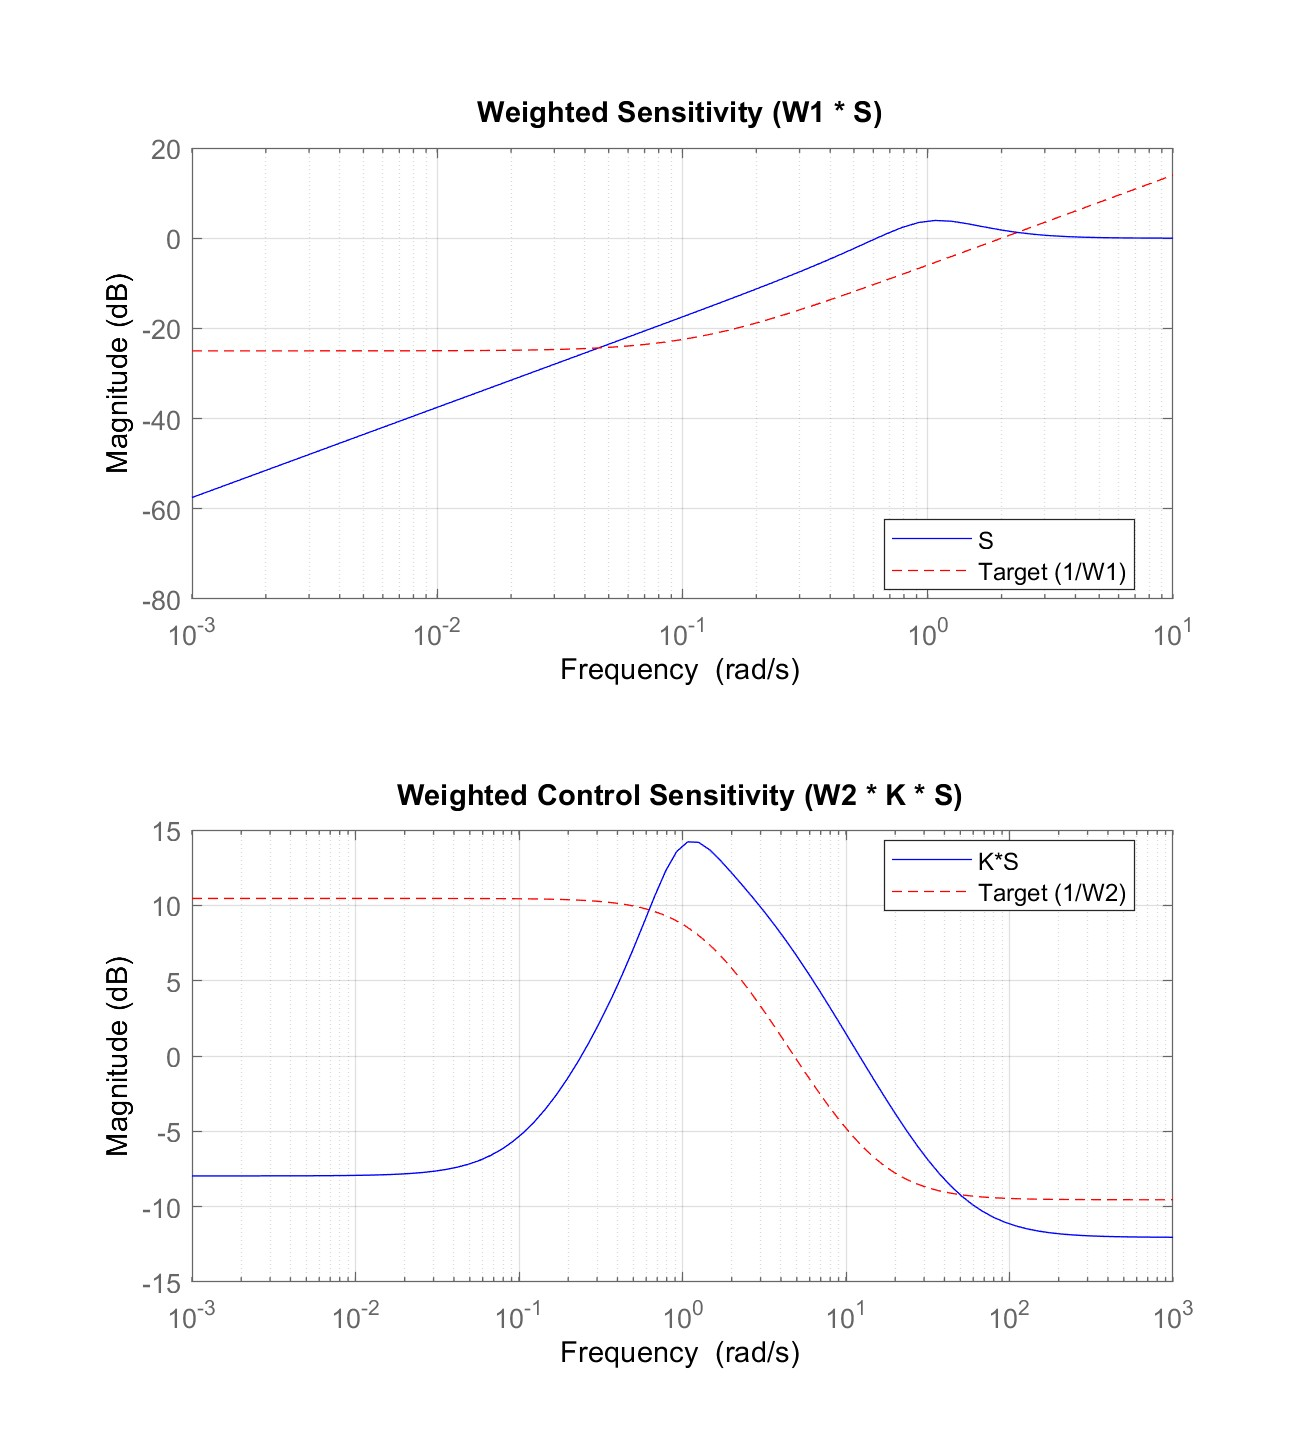
\includegraphics[scale=0.25]{images/Targets_K.jpg}
  \caption{Bode plots of the sensitivity and control sensitivity, compared to the shape they should have to satisfy nominal performance.}
  \label{fig:Targets_K}
\end{figure}

Consider now a time-delay in the transfer function $G_p$, as a first-order Padé approximation:

\begin{equation}
    G_p = \frac{h_p}{m_ps^2+c_ps+k_p}e^{-\tau_ps} \approx \frac{h_p}{m_ps^2+c_ps+k_p} \frac{1-\frac{\tau_p}{2}s}{1+\frac{\tau_p}{2}s}
\end{equation}

Where $\tau_p$ is an uncertain parameter with nominal value $\bar{\tau}$ and range $\left[0.07,0.13\right]$. 

The transfer function matrix has one input $d$ and two outputs ($\hat{y}$ and $\hat{u}$):

\begin{equation}
    \boldsymbol{G}_{\text{delay}} = \begin{bmatrix}
        W_1(1+G_pK)^{-1}\\  W_2K(1+G_pK)^{-1}
    \end{bmatrix}
\end{equation}

As shown in the code , this transfer function matrix can be converted into an uncertain state-space representation and through the \texttt{lftdata} command, it's possible to recover the $\boldsymbol{M}$-$\boldsymbol{\Delta}$ structure:

\begin{center}
    \begin{verbatim}
                [M_delay, Delta_delay] = lftdata(G_delay);
                n_delay = length(Delta_delay.NominalValue);
                M_11 = M_delay(1:n_delay, 1:n_delay);
    \end{verbatim}
\end{center}

The robust stability criterion shown in \ref{eq:robust_stability_req}, is not satisfied, so it's impossible to say whether this system is robustly stable with the small gain theorem. By using the less conservative procedure with the structured singular values shown in the previous snippet of code, the system is proved to be robustly stable even with the delay. If the reader is interested in the complete code, it can be found in the file \texttt{Ex\_2\_3\_1.m}.


\section{Sensitivity integrals}
The following proof was found on chapter 6.2 of \cite{Doy90}. The starting point is Lemma 3, which states that for every point $s_0=\sigma_0+j\omega$ with $\sigma_0>0$,

\begin{equation}
    \operatorname{log}|S_{\text{mp}}(s_0)|=\frac{1}{\pi}\int_{-\infty}^{\infty} \operatorname{log}{|S(j\omega)|}\frac{\sigma_0}{\sigma_0^2+(\omega-\omega_0)^2}d\omega.
\end{equation}
Where $S = S_\text{ap}S_\text{mp}$ where $S_\text{ap}$ is an all-pass function and $S_\text{mp}$ is a minimum phase function.
By taking $\omega_0=0$:

\begin{equation}
    \operatorname{log}|S_{\text{mp}}(\sigma_0)|=\frac{1}{\pi}\int_{-\infty}^{\infty} \operatorname{log}{|S(j\omega)|}\frac{\sigma_0}{\sigma_0^2+\omega^2}d\omega
\end{equation}

Or, equivalently:
\begin{equation}
    \int_{0}^{\infty} \operatorname{log}{|S(j\omega)|}\frac{\sigma_0^2}{\sigma_0^2+\omega^2}d\omega=\frac{\pi}{2} \sigma_0 \operatorname{log}|S_{\text{mp}}(\sigma_0)|
\end{equation}

Since $\lim_{\sigma_0\rightarrow \infty}{\frac{\sigma_0^2}{\sigma_0^2+\omega^2}}=1$ and $\lim_{\omega\rightarrow \infty}{\operatorname{log}{|S(j\omega)|}}=0$, the left hand converges to:

\begin{equation}
    \int_{0}^{\infty} \operatorname{log}{|S(j\omega)|}d\omega
\end{equation}

So, it remains to show that:

\begin{equation}
    \lim_{\sigma\rightarrow \infty}{\frac{\sigma}{2} \operatorname{log}\left|S_{\text{mp}}(\sigma)\right|}=(\operatorname{log}{e})\left(\sum\text{Re }p_i\right)
    \label{eq:claim}
\end{equation}

It's possible to write the non-minimum phase part as:
\begin{equation}
    S_\text{ap}(s) = \prod_{i}{\frac{s-p_i}{s+\bar{p}_i}}
\end{equation}

Since $L$ has a relative degree of at least 2:
\begin{equation}
    L(\sigma)\approx \frac{c}{\sigma^k} \quad \text{as }  \sigma \rightarrow \infty
\end{equation}
for some constant $c$ and some integer $k\geq2$. Thus, as $\sigma\rightarrow \infty$:

\begin{equation}
    \sigma\operatorname{ln}{S(\sigma)}=-\sigma\operatorname{ln}{1+L(\sigma)}\approx-\sigma\operatorname{ln}{\left(1+\frac{c}{\sigma^k}\right)}
\end{equation}

Now use the Maclaurin's series:
\begin{equation}
    \operatorname{1+x}=x-\frac{x^2}{2}+\dotsi
    \label{eq:maclaurin}
\end{equation}

to get:
\begin{equation}
    \sigma\operatorname{ln}{S(\sigma)}\approx-\sigma\left(\frac{c}{\sigma^k}-\dotsi \right)
\end{equation}

Which proves that:

\begin{equation}
    \lim_{\sigma\rightarrow\infty}{\sigma\operatorname{ln}{S(\sigma)}}=0
\end{equation}

Since $S_\text{mp}=S/S_\text{ap}$, to prove Eq. \ref{eq:claim}, it remains to show that:
\begin{equation}
    \lim_{\sigma\rightarrow \infty}{\frac{\pi}{2} \sigma \operatorname{ln}\left|\left[S_\text{ap}(\sigma)^{-1}\right]\right|}=\sum\text{Re }p_i
\end{equation}

Where:
\begin{equation}
    \operatorname{ln}{(S_\text{ap}(\sigma)^{-1})}=\operatorname{ln}{\prod_i{\frac{\sigma+\bar{p}_i}{\sigma-p_i}}}=\sum_i{\operatorname{ln}{\frac{\sigma+\bar{p}_i}{\sigma-p_i}}}
    \label{eq:last_claim}
\end{equation}

Let $p_i=x+jy$ and use Eq. \ref{eq:maclaurin} as follows:

\begin{align}
    \frac{\sigma}{2} \ln \left| \frac{\sigma + \bar{p}_i}{\sigma - p_i} \right| 
    &= \frac{\sigma}{2} \ln \left| \frac{1 + \bar{p}_i \sigma^{-1}}{1 - p_i \sigma^{-1}} \right| \\
    &= \frac{\sigma}{4} \ln \frac{(1 + x\sigma^{-1})^2 + (y\sigma^{-1})^2}{(1 - x\sigma^{-1})^2 + (y\sigma^{-1})^2} \\
    &= \frac{\sigma}{4} \left\{ \ln[(1 + x\sigma^{-1})^2 + (y\sigma^{-1})^2] - \ln[(1 - x\sigma^{-1})^2 + (y\sigma^{-1})^2] \right\} \\
    &= \frac{\sigma}{4} \left\{ 2\frac{x}{\sigma} + 2\frac{x}{\sigma} + \cdots \right\} \\
    &= x + \cdots \\
    &= \text{Re} p_i + \cdots.
\end{align}

Letting $\sigma\rightarrow\infty$ gives:

\begin{equation}
    \lim_{\sigma\rightarrow\infty}{\left|\frac{\sigma+\bar{p}_i}{\sigma-p_i}\right|}=\text{Re }p_i
\end{equation}

Which proves Eq. \ref{eq:last_claim}. By putting every step together, it's proved that:
\begin{equation}
    \int_{0}^{\infty}\operatorname{log}{|S(j\omega)|d\omega}=\pi(\operatorname{log}{e})\left(\sum_{i}^{N_p}\text{Re }p_i\right)
\end{equation}

Or, by the property of logarithms:
\begin{equation}
    \int_{0}^{\infty}\operatorname{ln}{|S(j\omega)|d\omega}=\pi\left(\sum_{i}^{N_p}\text{Re }p_i\right)
\end{equation}

Which is the desired result (both for the base $10$ and natural logarithms).

Consider now the following statement from Lemma 2 of Chapter 6.2 of \cite{Doy90}:

\begin{quote}
    For each function $G$ consisting of stable and proper real rational transfer functions, there exist
an all-pass function $G_{ap}$ and a minimum-phase function $G_{mp}$ such that $G = G_{ap}G_{mp}$. The
factors are unique up to sign.
\end{quote}

There, the following proof is explained. 

Let $G_{ap}$ be the product of all factors of the form:

\begin{equation}
    \frac{s-s_0}{s+\bar{s_0}}
\end{equation}

where $s_0$ ranges over all zeros of $G$ in $\text{Re}(s)>0$, counting multiplicities. This is an all-pass filter because its magnitude is 1 anywhere on the imaginary axis. Then define:

\begin{equation}
    G_{mp}=\frac{G}{G_{ap}}
\end{equation}

Which completes the proof of existence by construction.
\vspace{0.5cm}

Suppose $G$ has two factorizations, such that:

\begin{equation}
    G = G_{ap1} G_{mp1} = G_{ap2} G_{mp2}    
\end{equation}

where $G_{ap1}$ and $G_{ap2}$ are all-pass functions, and $G_{mp1}$ and $G_{mp2}$ are minimum-phase functions. 

A function $H$ is defined as:
\begin{equation}
    H = \frac{G_{ap1}}{G_{ap2}} = \frac{G_{mp2}}{G_{mp1}}
\end{equation}

Since $H$ is the ratio of two all-pass functions, it satisfies $|H(j\omega)| = 1\quad \forall\omega$ and is a rational all-pass function itself. Rational all-pass function have their zeros located at the mirror images of their poles across the imaginary axis, as defined for the function $G_{ap}$ in the previous part.

Moreover, since $H$ is the ratio of two minimum-phase functions, it's also a minimum-phase function. By definition, a minimum-phase function cannot have any poles or zeros in the open right half-plane. The previous requirement, though imposed symmetry, so it's also impossible for it to have poles in the left half-plane either. It's also impossible to have poles/zeros in the origin without breaking the norm constraint.

Finally, $H$ is a rational function with no poles, no zeros, and with unit norm, which means it has to be: $H(s)=\pm1$, which proves the factors are unique up to the sign.



\chapter{Coprime factorization and Youla Parametrization}

\section{HIMAT example system analysis}
To compute the Smith and Smith-McMillan forms of the reduced system, the following steps were performed:

\begin{enumerate}
    \item Computing the common denominator: This is the characteristic polynomial of matrix $\boldsymbol{A}_\text{red}$:
    \begin{equation}
        d(s) = \det(s\boldsymbol{I} - \boldsymbol{A}_\text{red})
    \end{equation}
    Whose roots are the poles of the system.

    \item Conversion to polynomial matrix: The MATLAB function \texttt{smithForm} requires a polynomial input, but the system's transfer function is rational. Therefore, the transfer function $\boldsymbol{G}(s)$ is converted into the polynomial matrix $\boldsymbol{N}(s)$ by clearing the denominators:
    \begin{equation}
        \boldsymbol{N}(s) = \boldsymbol{G}(s) \cdot d(s)
    \end{equation}

    \item Smith Normal Form:
    The Smith Normal Form of the $\boldsymbol{N}(s)$ is computed through the function \texttt{smithForm}, which returns:
    \begin{equation}
        \boldsymbol{S}(s) = \boldsymbol{U}(s) \boldsymbol{N}(s) \boldsymbol{V}(s) = \text{diag}(\gamma'_1(s), \dots, \gamma'_r(s))
    \end{equation}
    where $\gamma'_i(s)$ are the invariant polynomials such that $\gamma'_i(s)$ divides $\gamma'_{i+1}(s)$.

    \item Smith-McMillan Form:
    The Smith-McMillan form $\boldsymbol{M}(s)$ is obtained by dividing the Smith form back by the common denominator:
    \begin{equation}
        \boldsymbol{M}(s) = \frac{\boldsymbol{S}(s)}{d(s)} = \text{diag}\left( \frac{\gamma_1(s)}{\beta_1(s)}, \dots, \frac{\gamma_r(s)}{\beta_r(s)} \right)
    \end{equation}
    where $\gamma_i(s)$ and $\beta_i(s)$ are coprime polynomials. In particular:
    \begin{itemize}
        \item The roots of $\prod \gamma_i(s)$ are the transmission zeros.
        \item The roots of $\prod \beta_i(s)$ are the system poles.
    \end{itemize}
\end{enumerate}

By looking at the zeros and poles computed this way, it's clear that the pole-zeros cancellations didn't happen due to numerical error. The poles and zeros found through the roots of the numerator and denominator of the Smith-McMillan form are shown in Table \ref{tab:system_comparison}, together with the actual poles and zeros of the reduced system, computed using \texttt{tzero} and \texttt{pole}. The poles are repeated twice, and that is because they should have canceled with "fake" zeros which show up only because of small numerical differences that prevent cancellations. Notice also how all three systems are unstable, as they have poles in the open right half-plane.

\begin{table}[h]
\centering
\begin{tabular}{|c|c|c|c|}
\hline
\textbf{Metric} & \textbf{Original System} & \textbf{Reduced System} & \textbf{Smith-McMillan Form} \\ \hline
\textbf{Zeros} & -0.0210 & \begin{tabular}{@{}c@{}} -0.0272 \\ 58.2846 \end{tabular} & \begin{tabular}{@{}c@{}} -3.8830, -0.4742 \\ -0.0272, 0.5937 \\ 0.6951, 58.2846 \end{tabular} \\ \hline
\textbf{Poles} & \begin{tabular}{@{}c@{}} -0.2578 \\ $0.6898 \pm 0.2488i$ \\ -5.6757 \\ -30.0000 (x2) \end{tabular} & \begin{tabular}{@{}c@{}} -3.8830 \\ -0.4742 \\ 0.5937 \\ 0.6951 \end{tabular} & \begin{tabular}{@{}c@{}} -3.8830 (x2) \\ -0.4742 (x2) \\ 0.5937 (x2) \\ 0.6951 (x2) \end{tabular} \\ \hline
\end{tabular}
\caption{Comparison of Poles/Zeros: Original, Reduced, and Smith-McMillan Results}
\label{tab:system_comparison}
\end{table}

The Singular Value plots of the transfer function of the original system and the reduced system are shown in Figure \ref{fig:Model_reduction_accuracy}. At low frequency, they are very close to each other, showing that the approximation is good. The difference is at higher frequency, where they are more separated. This is expected from a lower-order approximation, since it's important that the approximation is valid only within a certain bandwidth.

\begin{figure}[htb]
  \centering
  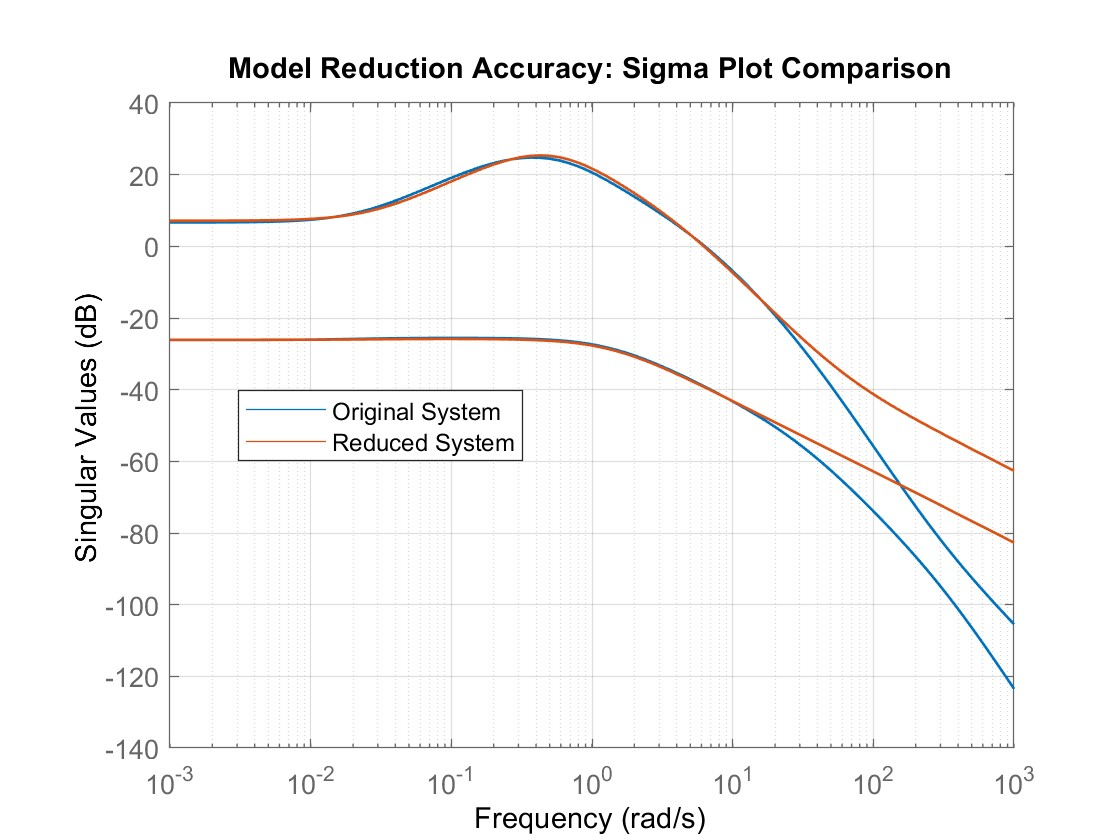
\includegraphics[scale=0.3]{images/Model_reduction_accuracy.jpg}
  \caption{Accuracy of the reduced model.}
  \label{fig:Model_reduction_accuracy}
\end{figure}


\section{Coprime factorization}
A procedure to find a doubly-coprime factorization of a system $\boldsymbol{G}$ is available in \cite{Fra87}. This factorization is formed by four matrices $\boldsymbol{N, M, \tilde{N}}$ and $\tilde{\boldsymbol{M}}$ that satisfy the Eq. \ref{eq:G_NM} and Eq. \ref{eq:Bezout's identity}.
\begin{equation}
    \boldsymbol{G} = \boldsymbol{N M}^{-1} = \boldsymbol{\tilde{M}}^{-1} \boldsymbol{\tilde{N}}
    \label{eq:G_NM}
\end{equation}

\begin{equation}    
    \begin{bmatrix} 
    \boldsymbol{\tilde{X}} & -\boldsymbol{\tilde{Y}} \\ 
    -\boldsymbol{\tilde{N}} & \boldsymbol{\tilde{M}} 
    \end{bmatrix}
    \begin{bmatrix} 
    \boldsymbol{M} & \boldsymbol{Y} \\ 
    \boldsymbol{N} & \boldsymbol{X} 
    \end{bmatrix} 
    = \boldsymbol{I}
    \label{eq:Bezout's identity}
\end{equation}

The procedure to find these matrices is the following.

After computing the transfer function of the reduced system through its state-space representation, it's necessary to define a real matrix $\boldsymbol{F}$ such that $\boldsymbol{A}_F:=\boldsymbol{A+BF}$ is stable. In order to do this, the MATLAB function \texttt{place} was used to place the poles of such system at $\begin{bmatrix}
    -2, & -5, & -8
\end{bmatrix}$.

Similarly, it's also necessary to define a matrix $\boldsymbol{H}$ such that $\boldsymbol{A}_H = \boldsymbol{A} + \boldsymbol{HC}$ is stable. In the same way as before, the poles were placed at $\begin{bmatrix}
    -2, & -5, & -8
\end{bmatrix}$. After defining the function $\boldsymbol{B}_H = \boldsymbol{B}+ \boldsymbol{HD}$, it's possible to find the matrices that define the matrices that compose the doubly-coprime factorization:

\begin{align*}
\mathbf{M}(s) &:= \left[ \begin{array}{c|c} \mathbf{A}_F & \mathbf{B} \\ \hline \mathbf{F} & \mathbf{I} \end{array} \right] &
\mathbf{N}(s) &:= \left[ \begin{array}{c|c} \mathbf{A}_F & \mathbf{B} \\ \hline \mathbf{C}_F & \mathbf{D} \end{array} \right] \\[1em]
\tilde{\mathbf{M}}(s) &:= \left[ \begin{array}{c|c} \mathbf{A}_H & \mathbf{H} \\ \hline \mathbf{C} & \mathbf{I} \end{array} \right] &
\tilde{\mathbf{N}}(s) &:= \left[ \begin{array}{c|c} \mathbf{A}_H & \mathbf{B}_H \\ \hline \mathbf{C} & \mathbf{D} \end{array} \right] \\[1.5em]
\mathbf{X}(s) &:= \left[ \begin{array}{c|c} \mathbf{A}_F & -\mathbf{H} \\ \hline \mathbf{C}_F & \mathbf{I} \end{array} \right] &
\mathbf{Y}(s) &:= \left[ \begin{array}{c|c} \mathbf{A}_F & -\mathbf{H} \\ \hline \mathbf{F} & \mathbf{0} \end{array} \right] \\[1em]
\tilde{\mathbf{X}}(s) &:= \left[ \begin{array}{c|c} \mathbf{A}_H & -\mathbf{B}_H \\ \hline \mathbf{F} & \mathbf{I} \end{array} \right] &
\tilde{\mathbf{Y}}(s) &:= \left[ \begin{array}{c|c} \mathbf{A}_H & -\mathbf{H} \\ \hline \mathbf{F} & \mathbf{0} \end{array} \right]
\end{align*}

To check whether this parametrization was correct, it was proved that these matrices respect Bezout's identity shown in Eq. \ref{eq:Bezout's identity}:

\begin{equation}
    \left\|\begin{bmatrix} 
    \boldsymbol{\tilde{X}} & -\boldsymbol{\tilde{Y}} \\ 
    -\boldsymbol{\tilde{N}} & \boldsymbol{\tilde{M}} 
    \end{bmatrix}
    \begin{bmatrix} 
    \boldsymbol{M} & \boldsymbol{Y} \\ 
    \boldsymbol{N} & \boldsymbol{X} 
    \end{bmatrix} 
    - \boldsymbol{I}\right\|_\infty=1.2073\cdot10^{-7}
\end{equation}

Which is an acceptable numerical error.



\section{Youla parametrization}
Once the doubly-coprime factorization of $\boldsymbol{G}$ is available, the set of all (proper-real-rational) controllers $\boldsymbol{K}$ stabilizing $\boldsymbol{G}$ is parametrized by the formulas:

\begin{align}
\boldsymbol{K} &= (\boldsymbol{Y} - \boldsymbol{M Q})(\boldsymbol{X} - \boldsymbol{N Q})^{-1} \\
  &= (\tilde{\boldsymbol{X}} - \boldsymbol{Q} \tilde{\boldsymbol{N}})^{-1} (\tilde{\boldsymbol{Y}} - \boldsymbol{Q} \tilde{\boldsymbol{M}})
\end{align}

\begin{equation}
    \boldsymbol{Q} \in \mathcal{RH}_{\infty}
\end{equation}

A stabilizing controller can be found, for example, by setting $\boldsymbol{Q}=\boldsymbol{0}$. Using the function \texttt{sigma}, it's possible to plot the singular values as function of the frequency. As in our case the system has two inputs and two outputs, we have two singular values both for the sensitivity transfer function and for the complementary sensitivity. The singular value plots are shown in Figure \ref{fig:SV_Sens} and Figure \ref{fig:SV_Comp}.

\begin{figure}[htb]
  \centering
  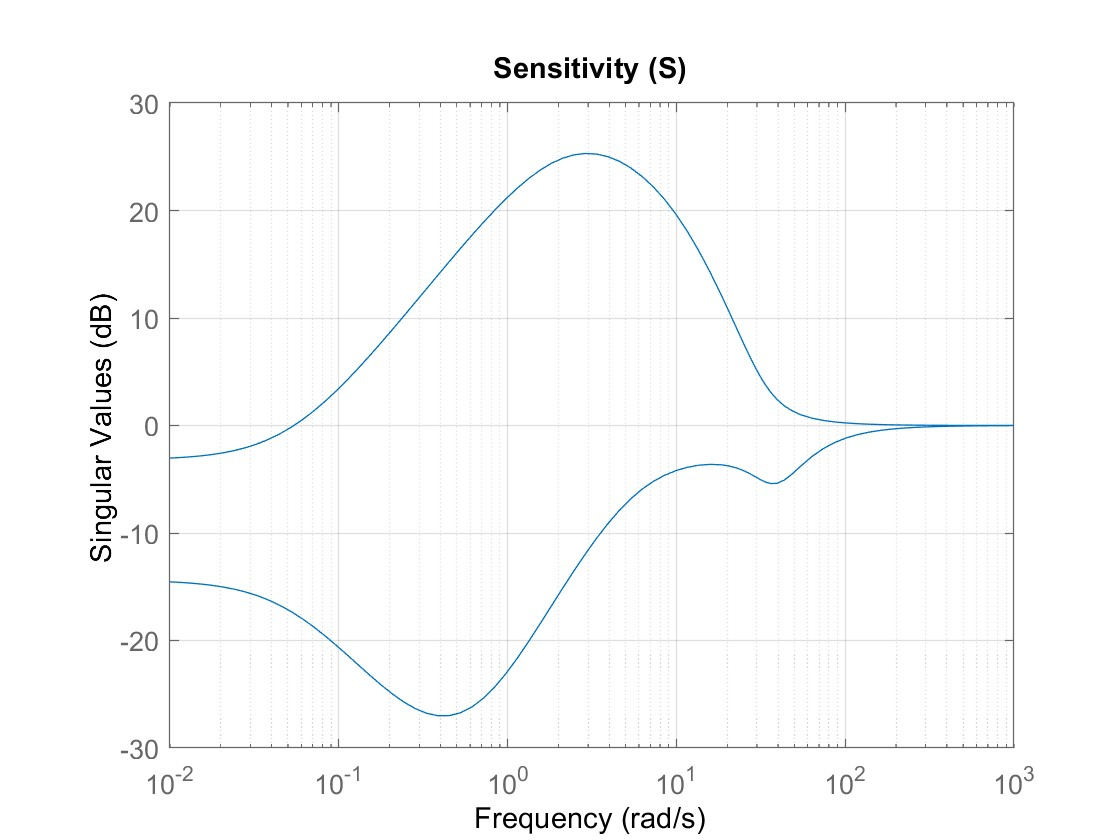
\includegraphics[scale=0.3]{images/Sensitivity_SV.jpg}
  \caption{Singular Value plot of the Sensitivity transfer function matrix $\boldsymbol{S}(s)$.}
  \label{fig:SV_Sens}
\end{figure}


\begin{figure}[htb]
  \centering
  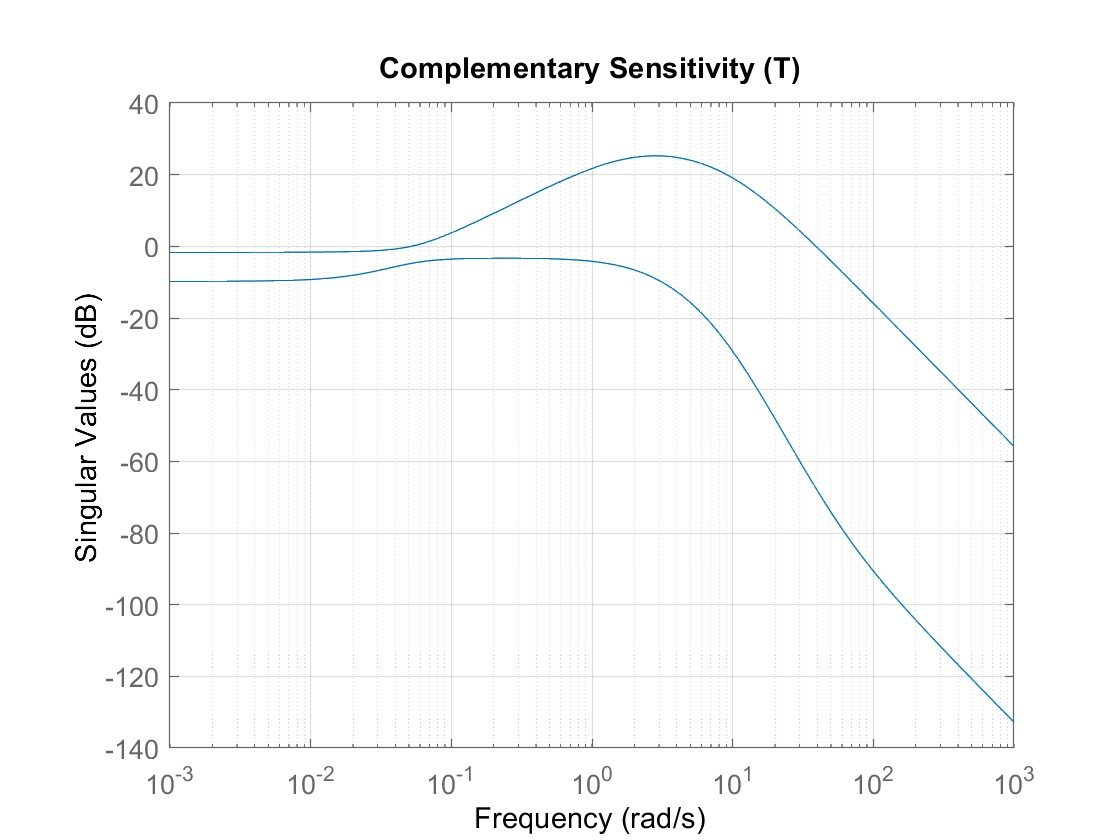
\includegraphics[scale=0.3]{images/Complementary_Sensitivity_SV.jpg}
  \caption{Singular Value plot of the Complementary Sensitivity transfer function matrix $\boldsymbol{T}(s)$.}
  \label{fig:SV_Comp}
\end{figure}

The step response of the stabilized system, instead, can be seen in Figure \ref{fig:stab_resp}. If necessary, it's possible to speed up the response of the system by moving the poles of $\boldsymbol{A}_F$ and $\boldsymbol{A}_H$ further to the left in the complex plane, at the expense of having a larger overshoot. All the code referenced in this chapter can be found in the file \texttt{Ex\_2\_4.m}.

\begin{figure}[htb]
  \centering
  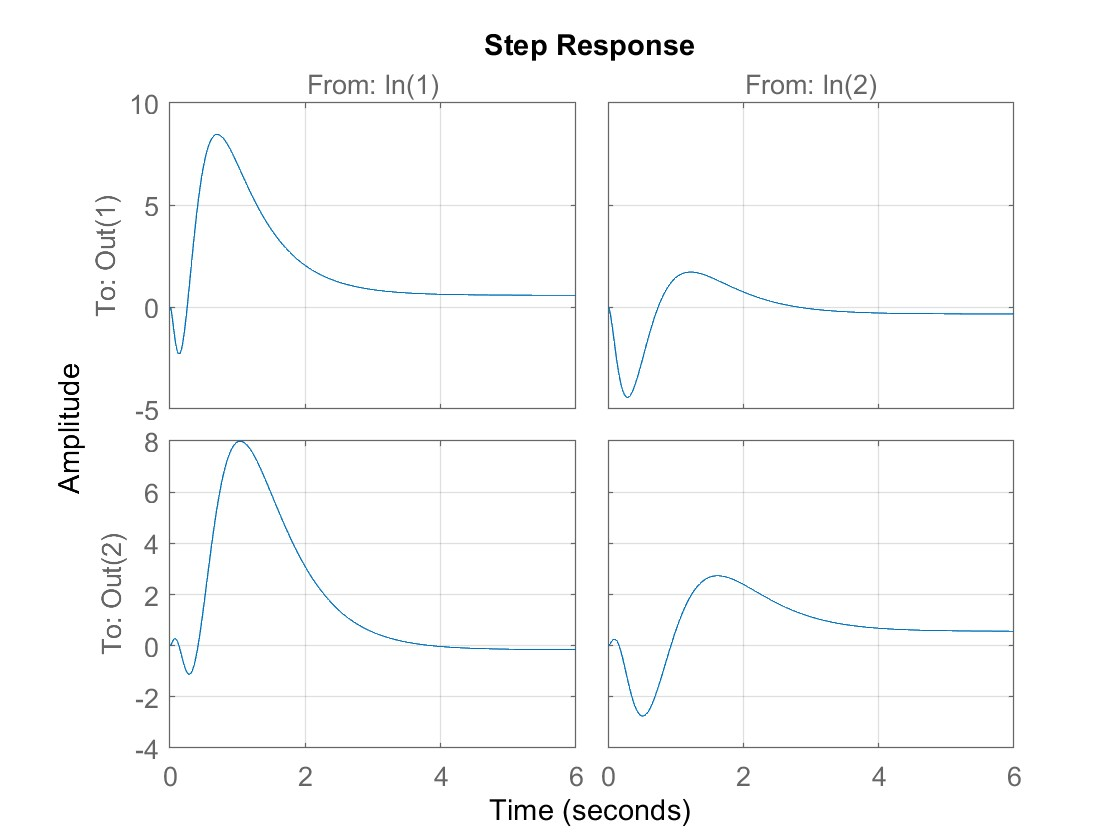
\includegraphics[scale=0.3]{images/Youla_system_response.jpg}
  \caption{Response of the stabilized system.}
  \label{fig:stab_resp}
\end{figure}


\bibliographystyle{abbrv}
\bibliography{literature}

\end{document}